%%
%% CSD Assignment 1 - Final Technical Report
%% ACM "acmart" manuscript (single-column) style.
%% Items still to be completed by the author are marked with \todo{...}
%% and appear in red in the PDF. Search for "\todo" before submitting.
%%
\documentclass[manuscript,screen,review]{acmart}

\AtBeginDocument{%
  \providecommand\BibTeX{{Bib\TeX}}}

% This is a course assignment report, not an ACM publication.
\setcopyright{none}
\settopmatter{printacmref=false}
\renewcommand\footnotetextcopyrightpermission[1]{}
\acmConference[CSD Assignment 1]{Computer System Design}{2026}{India}

\usepackage{tabularx}
\usepackage{multirow}
\usepackage{algorithm}
\usepackage{algpseudocode}
\usepackage{listings}
\usepackage{tikz}
\usetikzlibrary{arrows.meta,positioning,shapes.geometric,shapes.multipart,fit,backgrounds,calc}
\usepackage{pgfplots}
\pgfplotsset{compat=1.18}
\definecolor{accent}{HTML}{1C6FD1}
\definecolor{deep}{HTML}{12304F}
\definecolor{ink2}{HTML}{4A5666}
\definecolor{soft}{HTML}{E6F0FB}
\definecolor{good}{HTML}{1E7A4C}
\definecolor{warnc}{HTML}{8A5A00}
\definecolor{bad}{HTML}{B3261E}
\definecolor{pond}{HTML}{FF3D71}
\definecolor{water}{HTML}{4A90D9}
\definecolor{soil}{HTML}{8A6D3B}
\newcommand{\code}[1]{\texttt{\small #1}}
\newcommand{\todo}[1]{\textcolor{red}{\textbf{[TODO: #1]}}}
\newcommand{\ok}{\textcolor{good}{\textbf{met}}}
\newcolumntype{Y}{>{\raggedright\arraybackslash}X}
\newcolumntype{P}[1]{>{\raggedright\arraybackslash}p{#1}}
\lstset{basicstyle=\ttfamily\scriptsize,columns=fullflexible,keepspaces=true,
  frame=single,rulecolor=\color{black!25},backgroundcolor=\color{soft!45},
  breaklines=true,showstringspaces=false,xleftmargin=4pt,xrightmargin=4pt}

\begin{document}

%% =================== TITLE & AUTHOR BLOCK =========================
\title{AI-based Village Pond Planning System}
\subtitle{CSD Assignment 1 -- Final Technical Report}

\author{Amandeeip Kammari}
\affiliation{%
  \institution{\todo{Institute / Department} \,(Roll No.\ 12341060)}
  \city{\todo{City}}
  \country{India}}
\email{amandeeip01@gmail.com}

\renewcommand{\shortauthors}{Kammari}

%% =================== ABSTRACT ======================================
\begin{abstract}
Village ponds are among the cheapest ways to harvest rainwater in rural India, but deciding
where to dig one, and how big to make it, normally needs a field survey and a hydrologist. We
present a web application that does this preliminary planning from free public data. Given a
village name or a map click, the server builds a 20\,m elevation model from global terrain
tiles (or from an uploaded KML contour map), routes surface flow with Priority-Flood
depression filling and the D8 algorithm, and identifies land available for excavation by
combining an OpenCV classifier on satellite imagery with OpenStreetMap exclusions and optional
government parcels. Candidate sites are scored on flow accumulation, slope, concavity and land
suitability, and a ranking algorithm returns up to five sites whose catchments are
hydrologically independent. Twenty years of daily CHIRPS rainfall drive a daily SCS Curve
Number runoff model, and each pond is sized to half of the 75\,\%-dependable annual runoff.
The system is a modular FastAPI monolith with SQLite, a three-level cache and a fallback chain
for every external service. It was validated against independent data (CHIRPS rainfall within
8.9\,\% of IMD normals; land classifier 92\,\% accurate, $\kappa=0.85$), covered by 35
automated tests, load-tested, and deployed on a college lab server, where system testing found
and fixed six defects that unit tests had missed. For Hiware Bazar (Maharashtra) it recommends
five ponds storing 121\,155\,m$^3$. A first analysis takes about 44\,s, dominated by the
rainfall download; a cached one takes 1.3\,s, and eight concurrent cached analyses complete in
1.3\,s each.
\end{abstract}

\keywords{Village Pond Planning, Geospatial Analysis, Rainwater Harvesting, Catchment
  Estimation, Web GIS, REST APIs}

\maketitle

%% =====================================================================
\section{Introduction}
\label{sec:intro}
Most of India's net sown area is rain-fed, and most of its rain falls in the four months of
the south-west monsoon. Small surface storages --- farm ponds, village tanks and the
\emph{Amrit Sarovars} built under national programmes~\cite{amritsarovar} --- hold this water
back for irrigation, livestock and groundwater recharge. Pond-based harvesting is effective
because it is cheap, built with local labour and machinery, and recharges aquifers while
storing surface water. A pond is only useful, however, if three early decisions are right:
\begin{enumerate}
  \item \textbf{Where?} On a drainage line that actually receives runoff, on gentle ground,
    and on land the village is allowed to dig --- usually panchayat or government land.
  \item \textbf{How much water will arrive?} This depends on catchment area, land cover, soil
    and the rainfall regime, \emph{including dry years}.
  \item \textbf{How big?} A pond much larger than its dependable inflow rarely fills; one much
    smaller wastes the catchment. Depth trades evaporation against excavation cost and safety.
\end{enumerate}

The goal of this assignment is a web application that analyses terrain and rainfall to
recommend suitable pond locations and to estimate catchment area, rainfall, runoff, pond depth
and storage capacity, all shown on an interactive map. Section~\ref{sec:requirements} states
the requirements, Section~\ref{sec:architecture} the architecture and design decisions,
Section~\ref{sec:methodology} the algorithms, and Section~\ref{sec:implementation} the
implementation and deployment. Section~\ref{sec:csd-themes} maps the design to Computer System
Design themes; Section~\ref{sec:results} presents the case study, validation, testing and
measured performance; Section~\ref{sec:discussion} discusses limitations.

\subsection{Motivation}
Choosing a pond site by hand is hard for four reasons. \emph{Terrain is subtle}: on the gently
sloping Deccan plateau a drainage line can be invisible on the ground, yet a few metres of
relief decide where water collects. \emph{Rainfall data is scattered}: IMD station records are
sparse, gridded products disagree (we measured one widely used dataset to be 92\,\% too wet in
a rain-shadow city), and an administrator rarely knows the dependable dry-year rainfall that
should govern design. \emph{Land ownership is not open}: finding land that is both free and
hydrologically useful needs local knowledge. \emph{Sizing needs a runoff model}, which is
beyond most panchayat staff. An automated tool that turns a village name into a short,
quantified list of candidates lets an engineer spend field time verifying a handful of good
options instead of searching a whole village.

\subsection{Scope of the Project}
The system \textbf{does}: find a village by name or map click; build a terrain model from an
elevation service or an uploaded KML/KMZ contour map; display satellite imagery, contours,
drainage and land cover; identify land available for excavation; recommend up to five ranked
pond sites with independent catchments (or evaluate a site chosen by the user); delineate each
catchment; retrieve 5--40 years of daily rainfall; estimate runoff; recommend pond dimensions,
storage, earthwork and water losses; and save, list and export analyses.

The system \textbf{does not}: perform structural or geotechnical design of embankments,
inlets or spillways; determine legal land ownership (it can only use parcels supplied by the
administrator); model groundwater, measured infiltration or water quality; estimate costs; or
replace a field survey. It is a \emph{pre-feasibility} tool.

\subsection{Contributions}
\begin{itemize}
  \item An end-to-end pipeline from a place name to ranked, dimensioned pond sites using only
    free public data and no GIS server software.
  \item A ranking algorithm (Algorithm~\ref{alg:rank}) that guarantees independent
    alternatives, and a land-availability model that fuses image classification,
    OpenStreetMap and user parcels.
  \item A resilient service design --- caching, fallbacks, a circuit breaker and retries ---
    driven by load testing and a real deployment on an unreliable campus network.
  \item A quantitative validation of every data source, which changed the system's default
    rainfall dataset, and a test suite that includes regression tests for every defect found.
\end{itemize}

%% =====================================================================
\section{Problem Statement and Requirements}
\label{sec:requirements}
Given a location in rural India, the system must recommend where a rainwater-harvesting pond
should be excavated and how large it should be, and justify the recommendation with terrain,
land, rainfall and runoff evidence on a map. Table~\ref{tab:requirements} maps each functional
requirement of the brief to the module that implements it and the output that shows it.

\begin{table}[h]
  \caption{Functional requirements and where they are implemented}
  \label{tab:requirements}
  \small
  \begin{tabularx}{\linewidth}{@{}P{3.3cm}P{3.4cm}YP{3.0cm}@{}}
    \toprule
    Requirement & Implemented in & How & Visible as \\
    \midrule
    Satellite imagery display & \code{geocode.py}, \code{static/app.js} & Nominatim village search; Esri World Imagery basemap with labels & Satellite map, search box \\
    Contour map visualization & \code{layers.py}, \code{kml\_parser.py} & Contours traced from the DEM with OpenCV, or uploaded KML contours; relief overlay & Contour and relief layers \\
    Available-land identification & \code{landcover.py} & OpenCV classification + OpenStreetMap exclusions + parcels + slope + sea mask & Available-land and land-cover layers \\
    Catchment area estimation & \code{hydrology.py} & Priority-Flood, D8, accumulation, reverse traversal, boundary tracing & Catchment polygon, area, relief \\
    Historical rainfall query & \code{rainfall.py} & CHIRPS (ClimateSERV); fallback Open-Meteo ERA5, then NASA POWER & Rainfall tab, charts \\
    Runoff volume estimation & \code{runoff.py} & Daily SCS Curve Number with antecedent moisture; rational-method check & Runoff tab \\
    Pond depth / storage recommendation & \code{pond.py}, \code{design.py} & Site scoring and ranking; frustum sized to dependable runoff & Pond tab, cross-section, footprint \\
    Combined overlay / results view & \code{static/}, \code{pipeline.py} & Leaflet layers, Chart.js, candidate table, exports & Map + sidebar, JSON/GeoJSON \\
    \bottomrule
  \end{tabularx}
\end{table}

\subsection{Non-Functional Requirements}
Table~\ref{tab:nfr} lists the non-functional requirements we set, each with a measurable
target, and what was measured (Section~\ref{sec:perf}).

\begin{table}[h]
  \caption{Non-functional requirements: targets and measured results}
  \label{tab:nfr}
  \small
  \begin{tabularx}{\linewidth}{@{}P{2.3cm}YYP{1.1cm}@{}}
    \toprule
    Quality & Target & Measured & Status \\
    \midrule
    Performance & First analysis of a new village $\le$ 60\,s; repeat $\le$ 5\,s; light endpoints $<$ 50\,ms & 44.2\,s first; 1.3\,s repeat; health 2.4\,ms median, cached rainfall 8\,ms & \ok \\
    Scalability & $\ge$ 8 concurrent analyses on one instance without degrading results & 8 concurrent cached analyses: 1.32\,s median, 1.35\,s max (after the fixes in Section~\ref{sec:loadtest}) & \ok \\
    Availability & Failure of any one external service degrades, never aborts, and is reported & Fallback for every source; degradations listed in \code{warnings}; verified on a network where four services failed intermittently & \ok \\
    Usability & Analysis from a village name alone; keyboard and screen-reader use; WCAG AA contrast; current desktop browsers & Only \code{lat}/\code{lon} required; ARIA tabs, focus, skip link; 5.6:1 text contrast & \ok \\
    Security & Validate all input; 25\,MB upload cap; no secrets in the repository; external calls from the server only & Pydantic validation; size check; full git history scanned before publishing & \ok \\
    Portability & pip-installable without GIS servers; container image; free hosting & Runs on macOS and Ubuntu 24.04 lab server; Dockerfile and Render blueprint & \ok \\
    Transparency & Every number traceable to data and method & Response carries sources, methods, parameters, timings, warnings & \ok \\
    \bottomrule
  \end{tabularx}
\end{table}

%% =====================================================================
\section{System Architecture and High-Level Design}
\label{sec:architecture}
The system is a three-tier web application (Figure~\ref{fig:architecture}). The
\emph{client} is a static single-page application (HTML, CSS, JavaScript with Leaflet and
Chart.js). The \emph{application server} is one FastAPI process holding all analysis logic in
a pipeline of independent modules. The \emph{persistence tier} is an SQLite database (saved
analyses and an API-response cache) plus a disk cache of map tiles. The \emph{external API
layer} consists of seven free public services, which only the server calls; this lets it set
proper User-Agent headers, cache responses, and stay within fair-use limits.

\begin{figure}[h]
  \centering
  \resizebox{\linewidth}{!}{%
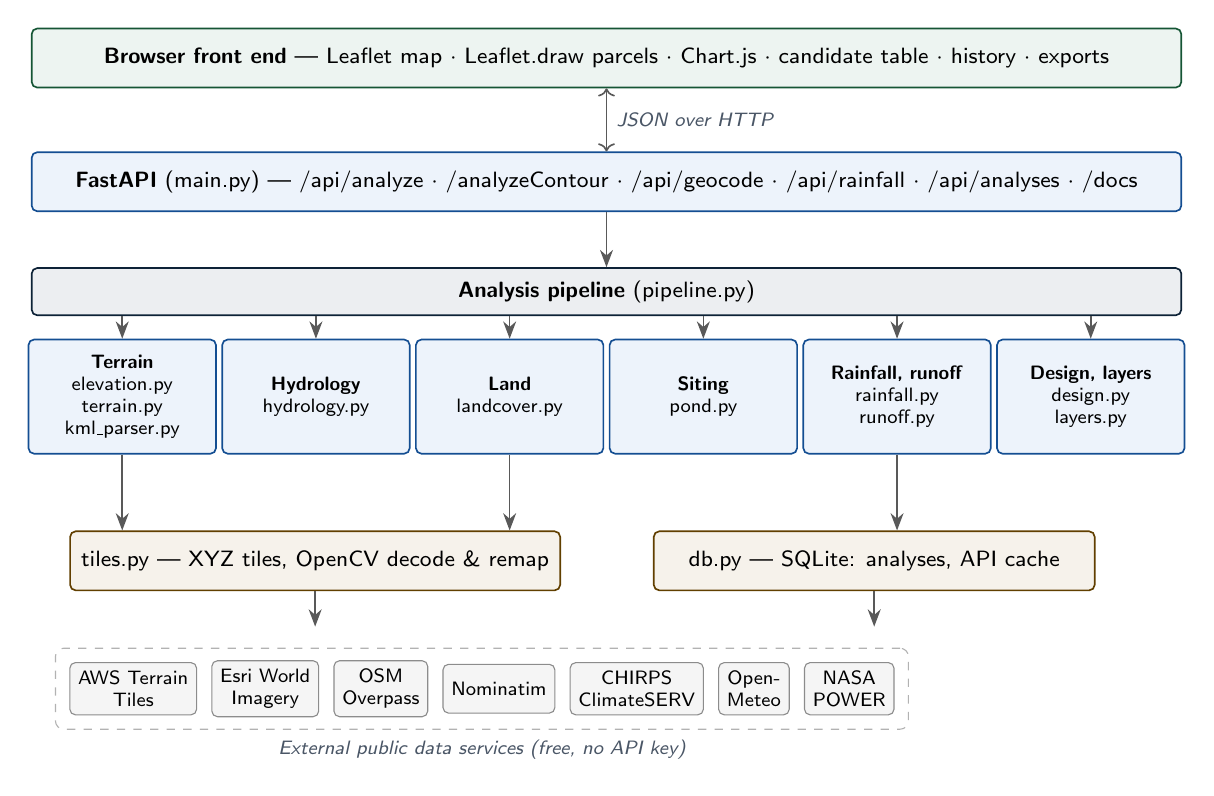
\begin{tikzpicture}[
  font=\sffamily\footnotesize,
  box/.style={draw=#1!70!black,fill=#1!8,rounded corners=2pt,minimum height=0.75cm,align=center,inner sep=4pt,line width=0.6pt},
  box/.default=accent,
  ext/.style={draw=black!45,fill=black!4,rounded corners=2pt,minimum height=0.62cm,align=center,inner sep=3pt,font=\sffamily\scriptsize},
  arr/.style={-{Stealth[length=2.2mm]},line width=0.6pt,color=black!65},
  lbl/.style={font=\sffamily\scriptsize\itshape,color=ink2}]
% Front end
\node[box=good,minimum width=14.6cm] (fe) at (0,0) {\textbf{Browser front end} --- Leaflet map $\cdot$ Leaflet.draw parcels $\cdot$ Chart.js $\cdot$ candidate table $\cdot$ history $\cdot$ exports};
% API
\node[box,minimum width=14.6cm,below=0.8cm of fe] (api) {\textbf{FastAPI} (main.py) --- /api/analyze $\cdot$ /analyzeContour $\cdot$ /api/geocode $\cdot$ /api/rainfall $\cdot$ /api/analyses $\cdot$ /docs};
\draw[arr,<->] (fe) -- node[right,lbl]{JSON over HTTP} (api);
% pipeline
\node[box=deep,minimum width=14.6cm,minimum height=0.6cm,below=0.7cm of api] (pipe) {\textbf{Analysis pipeline} (pipeline.py)};
\draw[arr] (api) -- (pipe);
% modules
\def\y{-4.3}
\tikzset{mod/.style={box,minimum width=2.3cm,text width=2.1cm,minimum height=1.45cm,font=\sffamily\scriptsize}}
\node[mod] (terr) at (-6.15,\y) {\textbf{Terrain}\\elevation.py\\terrain.py\\kml\_parser.py};
\node[mod] (hyd)  at (-3.69,\y) {\textbf{Hydrology}\\hydrology.py};
\node[mod] (land) at (-1.23,\y) {\textbf{Land}\\landcover.py};
\node[mod] (site) at (1.23,\y) {\textbf{Siting}\\pond.py};
\node[mod] (rain) at (3.69,\y) {\textbf{Rainfall, runoff}\\rainfall.py\\runoff.py};
\node[mod] (des)  at (6.15,\y) {\textbf{Design, layers}\\design.py\\layers.py};
\foreach \m in {terr,hyd,land,site,rain,des} \draw[arr] (pipe.south -| \m.north) -- (\m.north);
% infra
\node[box=warnc,minimum width=5.9cm,anchor=north] (tiles) at (-3.7,-6.0) {tiles.py --- XYZ tiles, OpenCV decode \& remap};
\node[box=warnc,minimum width=5.6cm,anchor=north] (db) at (3.4,-6.0) {db.py --- SQLite: analyses, API cache};
\draw[arr] (terr.south) -- (terr.south |- tiles.north);
\draw[arr] (land.south) -- (land.south |- tiles.north);
\draw[arr] (rain.south) -- (rain.south |- db.north);
% external
\node[ext,below=0.9cm of tiles.south west,anchor=north west] (e1) {AWS Terrain\\Tiles};
\node[ext,right=0.18cm of e1] (e2) {Esri World\\Imagery};
\node[ext,right=0.18cm of e2] (e3) {OSM\\Overpass};
\node[ext,right=0.18cm of e3] (e4) {Nominatim};
\node[ext,right=0.18cm of e4] (e5) {CHIRPS\\ClimateSERV};
\node[ext,right=0.18cm of e5] (e6) {Open-\\Meteo};
\node[ext,right=0.18cm of e6] (e7) {NASA\\POWER};
\begin{scope}[on background layer]
  \node[draw=black!30,dashed,rounded corners=3pt,fit=(e1)(e7),inner sep=5pt,label={[lbl]below:External public data services (free, no API key)}] {};
\end{scope}
\draw[arr] (tiles.south) -- ++(0,-0.45);
\draw[arr] (db.south) -- ++(0,-0.45);
\end{tikzpicture}
  }
  \caption{High-level system architecture. Arrows show the direction of calls. Only the
  server talks to external services, and their responses are cached.}
  \label{fig:architecture}
  \Description{Layered diagram. At the top, the browser front end (Leaflet map, Leaflet.draw,
  Chart.js, candidate table, history, exports) exchanges JSON over HTTP with the FastAPI
  application (main.py), which calls the analysis pipeline (pipeline.py). The pipeline calls
  six module groups: terrain, hydrology, land, siting, rainfall and runoff, and design and
  layers. Terrain and land use tiles.py; rainfall uses db.py (SQLite). At the bottom are the
  external services: AWS Terrain Tiles, Esri World Imagery, OSM Overpass, Nominatim, CHIRPS
  ClimateSERV, Open-Meteo and NASA POWER.}
\end{figure}

Figure~\ref{fig:flow} shows the processing stages of one analysis. The two inputs --- a
village location or an uploaded contour map --- converge on a common in-memory DEM, after
which the pipeline is identical, so a new terrain source can be added without touching the
hydrology. Figure~\ref{fig:seq} shows the same request as a sequence over time: the slow
rainfall download (two ten-year CHIRPS chunks) runs in parallel with the evapotranspiration
download, and on a repeat request every external call is served from a cache.

\begin{figure}[h]
  \centering
  \resizebox{\linewidth}{!}{%
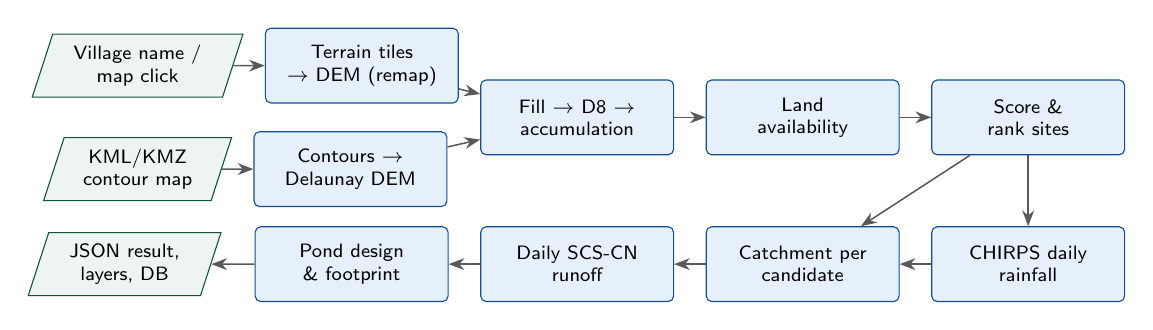
\begin{tikzpicture}[
  font=\sffamily\scriptsize,node distance=0.32cm and 0.4cm,
  st/.style={draw=accent!70!black,fill=soft,rounded corners=2pt,align=center,minimum width=2.45cm,minimum height=0.95cm,inner sep=2pt},
  io/.style={draw=good!70!black,fill=good!8,trapezium,trapezium left angle=72,trapezium right angle=108,align=center,minimum height=0.8cm,inner sep=2pt},
  arr/.style={-{Stealth[length=2mm]},line width=0.55pt,color=black!65}]
\node[io] (in1) {Village name /\\map click};
\node[io,below=0.5cm of in1] (in2) {KML/KMZ\\contour map};
\node[st,right=of in1] (dem1) {Terrain tiles\\$\rightarrow$ DEM (remap)};
\node[st,right=of in2] (dem2) {Contours $\rightarrow$\\Delaunay DEM};
\node[st,right=1.9cm of $(in1)!0.5!(in2)$,xshift=2.45cm] (hyd) {Fill $\rightarrow$ D8 $\rightarrow$\\accumulation};
\node[st,right=of hyd] (land) {Land\\availability};
\node[st,right=of land] (rank) {Score \&\\rank sites};
\node[st,below=0.9cm of rank] (rain) {CHIRPS daily\\rainfall};
\node[st,left=of rain] (catch) {Catchment per\\candidate};
\node[st,left=of catch] (run) {Daily SCS-CN\\runoff};
\node[st,left=of run] (des) {Pond design\\\& footprint};
\node[io,left=0.55cm of des] (out) {JSON result,\\layers, DB};
\draw[arr] (in1) -- (dem1); \draw[arr] (in2) -- (dem2);
\draw[arr] (dem1) -- (hyd); \draw[arr] (dem2) -- (hyd);
\draw[arr] (hyd) -- (land); \draw[arr] (land) -- (rank);
\draw[arr] (rank) -- (catch); \draw[arr] (rank) -- (rain);
\draw[arr] (rain) -- (catch);
\draw[arr] (catch) -- (run); \draw[arr] (run) -- (des); \draw[arr] (des) -- (out);
\end{tikzpicture}
  }
  \caption{Processing stages of one analysis. Rainfall is fetched once, at the top site, and
  shared by all candidates.}
  \label{fig:flow}
  \Description{Flow chart. A village name or map click leads to terrain tiles and a DEM; a
  KML/KMZ contour map leads to a Delaunay DEM. Both feed fill, D8 and accumulation, then land
  availability, then scoring and ranking of sites. Ranking feeds both the CHIRPS rainfall
  download and catchment delineation per candidate; these lead to daily SCS-CN runoff, pond
  design and footprint, and finally the JSON result, map layers and database record.}
\end{figure}

\begin{figure}[h]
  \centering
  \resizebox{\linewidth}{!}{%
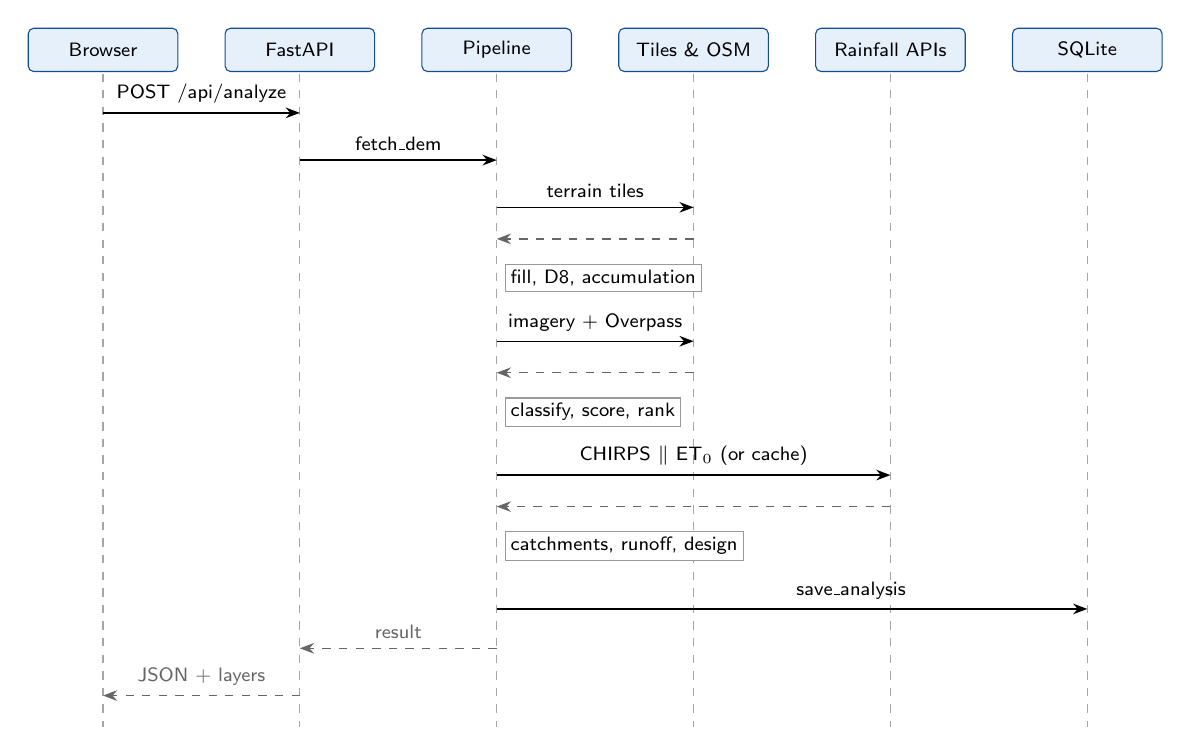
\begin{tikzpicture}[font=\sffamily\scriptsize,
  life/.style={draw=black!35,dashed},
  msg/.style={-{Stealth[length=1.8mm]},line width=0.5pt},
  ret/.style={-{Stealth[length=1.8mm]},dashed,line width=0.5pt,color=black!60},
  hd/.style={draw=accent!70!black,fill=soft,rounded corners=2pt,minimum width=1.9cm,minimum height=0.55cm,align=center}]
\foreach \x/\n/\t in {0/U/Browser,2.5/A/FastAPI,5/P/Pipeline,7.5/T/Tiles \& OSM,10/R/Rainfall APIs,12.5/D/SQLite}{
  \node[hd] (\n) at (\x,0) {\t};
  \draw[life] (\x,-0.3) -- (\x,-8.6);}
\tikzset{note/.style={draw=black!40,fill=white,anchor=west,font=\sffamily\scriptsize,inner sep=2pt}}
\draw[msg] (0,-0.8) -- node[above]{POST /api/analyze} (2.5,-0.8);
\draw[msg] (2.5,-1.4) -- node[above]{fetch\_dem} (5,-1.4);
\draw[msg] (5,-2.0) -- node[above]{terrain tiles} (7.5,-2.0);
\draw[ret] (7.5,-2.4) -- (5,-2.4);
\node[note] at (5.1,-2.9) {fill, D8, accumulation};
\draw[msg] (5,-3.7) -- node[above]{imagery + Overpass} (7.5,-3.7);
\draw[ret] (7.5,-4.1) -- (5,-4.1);
\node[note] at (5.1,-4.6) {classify, score, rank};
\draw[msg] (5,-5.4) -- node[above,pos=0.5]{CHIRPS $\parallel$ ET$_0$ (or cache)} (10,-5.4);
\draw[ret] (10,-5.8) -- (5,-5.8);
\node[note] at (5.1,-6.3) {catchments, runoff, design};
\draw[msg] (5,-7.1) -- node[above,pos=0.6]{save\_analysis} (12.5,-7.1);
\draw[ret] (5,-7.6) -- node[above]{result} (2.5,-7.6);
\draw[ret] (2.5,-8.2) -- node[above]{JSON + layers} (0,-8.2);
\end{tikzpicture}
  }
  \caption{Sequence of one village analysis request.}
  \label{fig:seq}
  \Description{Sequence diagram with six lifelines: Browser, FastAPI, Pipeline, Tiles and OSM,
  Rainfall APIs, SQLite. The browser posts to /api/analyze; FastAPI asks the pipeline to fetch
  the DEM; the pipeline requests terrain tiles, then performs fill, D8 and accumulation;
  requests imagery and Overpass data, then classifies, scores and ranks; requests CHIRPS and
  ET0 in parallel or from cache; computes catchments, runoff and design; saves the analysis to
  SQLite; and returns JSON and layers to the browser.}
\end{figure}

\subsection{Technology Stack}
Table~\ref{tab:stack} lists the stack actually used.

\begin{table}[h]
  \caption{Technology stack}
  \label{tab:stack}
  \small
  \begin{tabularx}{\linewidth}{@{}P{2.6cm}P{4.4cm}Y@{}}
    \toprule
    Layer & Technology & Why \\
    \midrule
    Language, server & Python 3.12+, FastAPI 0.115, Uvicorn 0.34, Pydantic 2.10 & Typed request/response models give validation and OpenAPI docs for free; scientific Python ecosystem \\
    Numerics, imaging & NumPy 2.2, SciPy 1.15, OpenCV 5 (headless) & Vectorised grids; Delaunay interpolation; tile decoding, \code{remap}, contours, morphology, rasterisation \\
    Database & SQLite (standard library) & Small document store, single writer, zero administration \\
    Frontend & HTML/CSS/JS, Leaflet 1.9, Leaflet.draw 1.0, Chart.js 4.4 & No build step; small; the brief asks for a basic library \\
    Terrain data & AWS Terrain Tiles (SRTM/Copernicus $\sim$30\,m); fallback Open-Meteo elevation & Global, key-less, one request per 256$\times$256 tile, cacheable \\
    Imagery, map data & Esri World Imagery; OpenStreetMap Overpass and Nominatim & Free high-resolution imagery; buildings, roads, water, land use; place search \\
    Rainfall, ET$_0$ & CHIRPS v2.0 via ClimateSERV; fallback Open-Meteo ERA5, NASA POWER & Most accurate against IMD normals (Table~\ref{tab:valrain}) \\
    Testing & pytest 9, FastAPI TestClient, curl-based end-to-end and load scripts & Unit, API, system and load levels \\
    Deployment & Docker, Render blueprint; venv + Uvicorn on the lab server & Reproducible, free; works without Docker where unavailable \\
    \bottomrule
  \end{tabularx}
\end{table}

\paragraph{Deviations from the suggested stack.} The brief suggests IMD for rainfall. IMD
gridded rainfall is distributed as bulk files rather than through a query API, so CHIRPS was
chosen after validating three datasets against IMD station normals: NASA POWER was off by up to
$+92\,\%$ in the rain shadow, CHIRPS by 8.9\,\% on average. We did not use GDAL or a GIS
server: the required algorithms are small enough to implement directly in NumPy and OpenCV,
which keeps the system installable from pip wheels on free hosting. SQLite replaces a
client--server database because the data is a small document store with one writer process.

\subsection{Key Design Decisions}
Table~\ref{tab:decisions} records the main design choices with the alternatives we considered.

\begin{table}[h]
  \caption{Design decisions and rationale}
  \label{tab:decisions}
  \small
  \begin{tabularx}{\linewidth}{@{}P{3.0cm}P{3.2cm}Y@{}}
    \toprule
    Decision & Alternatives & Rationale \\
    \midrule
    FastAPI & Flask, Django & Pydantic models validate requests and generate the OpenAPI reference; async-capable; same schemas document and validate. \\
    NumPy/SciPy/OpenCV hydrology & GDAL, WhiteboxTools, GRASS & Installs from pip on any platform and on free hosting; every algorithm is visible and testable. \\
    Terrain tiles for the DEM & OpenTopography, point APIs & One request per tile; a point API would need 40\,000 queries per 200$\times$200 grid. \\
    Local equirectangular projection & UTM via \code{pyproj} & Distortion far below DEM error over a few km; avoids a PROJ dependency. \\
    CHIRPS default rainfall & ERA5, NASA POWER, IMD grids & Best agreement with IMD normals; IMD grids are files, not an API. \\
    Daily SCS-CN & Rational method, monthly balance & Captures storm-size non-linearity and antecedent moisture; standard in Indian watershed manuals. \\
    Rule-based OpenCV + OSM for land & Deep segmentation model & No labelled Indian village data; explainable; no GPU; 92\,\% accurate. \\
    Modular monolith & Microservices & One developer; stages exchange large in-memory arrays; one deployable unit. \\
    SQLite & PostgreSQL, MongoDB & Single writer, small data; isolated behind \code{db.py} so it can be swapped. \\
    \bottomrule
  \end{tabularx}
\end{table}

%% =====================================================================
\section{Methodology}
\label{sec:methodology}

\subsection{Terrain and Elevation Analysis}
\paragraph{Grid.} For a village centre $(\lambda_0,\varphi_0)$ and radius $R$ (default 2\,km)
the server lays out an $N\times N$ grid (default $N=200$, cell size $\Delta=2R/N=20$\,m) in a
local equirectangular projection,
\begin{equation}
x = R_E\cos\varphi_0\,(\lambda-\lambda_0)\tfrac{\pi}{180},\qquad
y = R_E\,(\varphi-\varphi_0)\tfrac{\pi}{180},\qquad R_E = 6\,371\,008.8\ \text{m}.
\end{equation}

\paragraph{Elevation.} AWS Terrain Tiles encode elevation in the RGB bytes of 256$\times$256
Web-Mercator PNG tiles:
\begin{equation}
z = 256R + G + B/256 - 32768\ \ [\text{m}].
\end{equation}
The tiles covering the grid are downloaded in parallel (8 threads), decoded with OpenCV,
stitched into a mosaic and sampled at every cell centre with \code{cv2.remap} (bilinear).
Decoding happens \emph{before} resampling, because interpolating the packed bytes would mix
the high and low bytes of neighbouring pixels and produce errors of hundreds of metres. If the
tile service fails, a 40$\times$40 lattice is queried from the Open-Meteo elevation API and
interpolated bicubically.

\paragraph{Contour-map input.} For an uploaded KML/KMZ map, each contour's elevation is
detected from coordinate $z$ values, \code{ExtendedData}, the placemark name or the folder name
(the first strategy covering 90\,\% of lines with varying values wins). Vertices are
interpolated linearly over their Delaunay triangulation, with nearest-neighbour fill outside
the convex hull.

\paragraph{Derived terrain.} Contours for display are traced from the DEM with
\code{cv2.findContours} at an automatic interval with major and minor lines; slope and plan
curvature come from finite differences; a colour-relief hillshade is rendered as a PNG overlay.

\paragraph{Sea mask.} Terrain tiles report the sea as a flat 0\,m surface with bathymetry
further out. A connected low region ($z\le 0.05$\,m) is marked as sea only if it contains at
least 0.25\,\% of the grid's cells as flat sea surface ($|z|\le0.05$\,m) or bathymetry
($z<-5$\,m). This excludes the sea and the shallow seabed joined to it, while keeping inland
land below sea level, such as the polders of Kuttanad, Kerala. An area that is mostly sea is
rejected.

\subsection{Catchment Area Delineation}
Catchments are derived with standard raster flow routing (Table~\ref{tab:algos}).

\begin{table}[h]
  \caption{Hydrology algorithms ($n$ = number of cells, 40\,000 by default)}
  \label{tab:algos}
  \small
  \begin{tabularx}{\linewidth}{@{}P{2.9cm}YP{2.0cm}@{}}
    \toprule
    Step & Method & Complexity \\
    \midrule
    Depression filling & Priority-Flood~\cite{barnes2014}: seed a min-heap with edge cells; pop the lowest; raise each unvisited neighbour to at least its level $+10^{-4}$\,m & $O(n\log n)$ \\
    Flow direction & D8~\cite{ocallaghan1984}: steepest distance-weighted drop $s_k=(z_c-z_k)/d_k$, $d_k\in\{1,\sqrt2\}\Delta$, as eight vectorised array shifts & $O(n)$ \\
    Flow accumulation & Visit cells in decreasing filled elevation, adding each count to its receiver & $O(n\log n)$ (sort) \\
    Catchment & Breadth-first traversal of the reversed D8 graph from the outlet & $O(n)$ \\
    Boundary & Collect cell edges between inside and outside, stitch into a ring, drop collinear vertices; area = cells $\times\Delta^2$ & $O(n)$ \\
    Edge inflow & Border cells draining inward flag all cells downstream of them & $O(n\log n)$ \\
    \bottomrule
  \end{tabularx}
\end{table}

Priority-Flood was chosen over iterative pit filling, which can be $O(n^2)$; the whole terrain
stage takes about 60\,ms. In village mode, cells whose catchment may extend beyond the map edge
are excluded from siting, so no reported catchment is truncated.

\paragraph{Available land.} Esri imagery is resampled to 5\,m and classified per pixel:
\emph{vegetation} where the Green--Red Vegetation Index $\mathrm{GRVI}=(G-R)/(G+R)$ exceeds an
Otsu threshold~\cite{otsu1979} clamped to $[0,0.10]$; \emph{built-up} where bright, highly
textured pixels (local s.d.\ over 15\,m above $\max(18, P_{90})$) reach a density of 0.30 over
40\,m; \emph{water} for dark, blue-dominant, smooth pixels; \emph{open land} otherwise.
Morphological opening and closing remove speckle. OpenStreetMap buildings (+20\,m), roads
(+4--30\,m by class), railways, rivers, water bodies, forest, settlements, institutions and
protected areas are excluded; grassland, scrub, village green or public-ownership tags are
\emph{preferred}; farmland is allowed at lower priority. Administrator parcels, when given,
restrict siting to them, and ground steeper than 8\textdegree{} is excluded.

\paragraph{Site scoring and ranking.} Candidates are available cells on the drainage network
(top 8\,\% of accumulation, relaxed to the 85th, 75th and 60th percentiles if available land
does not reach it). Each candidate $c$ is scored
\begin{equation}
S_c = 0.75\big(0.45\,\hat A_c + 0.35\,(1-\hat\theta_c) + 0.20\,\hat\kappa_c\big) + 0.25\,L_c,
\end{equation}
with $\hat A$ the min--max normalised $\log(1+\text{accumulation})$, $\hat\theta$ normalised
slope, $\hat\kappa$ normalised concavity and $L$ the land score. Taking the top five scores
would return five adjacent cells on one stream, so Algorithm~\ref{alg:rank} enforces spatial
separation and hydrological independence: no site lies upstream or downstream of another, so
their inflows can be summed without double counting. A user-chosen location is instead
snapped to the highest-accumulation cell within 60\,m and becomes rank 1.

\begin{algorithm}[t]
\caption{Ranking independent candidate sites}\label{alg:rank}
\begin{algorithmic}[1]
\Require score grid $S$, D8 directions $D$, number $n$, minimum separation $d_{\min}$
\State $\mathcal{A}\gets[\,]$; $\mathcal{M}\gets[\,]$ \Comment{accepted sites, their catchment masks}
\ForAll{cells $c$ in decreasing order of $S$}
  \State \textbf{if} $|\mathcal{A}|=n$ \textbf{then break}
  \State \textbf{if} $\exists a\in\mathcal{A}:\ \lVert c-a\rVert<d_{\min}$ \textbf{then continue} \Comment{too close}
  \State \textbf{if} $\exists m\in\mathcal{M}:\ m[c]$ \textbf{then continue} \Comment{$c$ upstream of an accepted site}
  \State $m_c\gets\textsc{Catchment}(D,c)$
  \State \textbf{if} $\exists a\in\mathcal{A}:\ m_c[a]$ \textbf{then continue} \Comment{$c$ downstream of an accepted site}
  \State append $c$ to $\mathcal{A}$ and $m_c$ to $\mathcal{M}$
\EndFor
\State \Return $\mathcal{A}$
\end{algorithmic}
\end{algorithm}

\paragraph{Assumptions and limitations.} D8 sends all flow to one neighbour and cannot model
divergent flow; the $\sim$30\,m source DEM cannot see bunds or drains narrower than about
30\,m; land availability is inferred, not legal ownership.

\subsection{Rainfall Data Integration}
Daily precipitation comes from CHIRPS v2.0~\cite{funk2015} (0.05\textdegree{},
satellite--gauge blend) through the ClimateSERV API, downloaded as two ten-year chunks in
parallel. If CHIRPS fails, the system falls back to Open-Meteo's ERA5
reanalysis~\cite{hersbach2020}, then to NASA POWER; transient network errors are retried with
back-off, definitive ones (e.g.\ HTTP 429) move straight to the next source. Reference
evapotranspiration comes from Open-Meteo (FAO-56 Penman--Monteith) or, from NASA POWER
temperatures, by Hargreaves--Samani~\cite{allen1998}:
\begin{equation}
\mathrm{ET}_0 = 0.0023\,(0.408R_a)\,(T_\text{mean}+17.8)\sqrt{T_\text{max}-T_\text{min}}.
\end{equation}
The default record is the last 20 complete years (2006--2025), configurable from 5 to 40. If
the administrator knows the local IMD normal $\bar P^\ast$, the daily series is scaled by
$\bar P^\ast/\bar P$, preserving the storm pattern while removing bias.

From the daily series the system computes the mean, median, standard deviation and
coefficient of variation of annual totals; the 75\,\%-dependable rainfall (25th percentile of
annual totals, equalled or exceeded three years in four); the driest and wettest years; rainy
days ($\geq$2.5\,mm, the IMD definition); the heaviest day; the June--September share; the
monthly climatology; and annual and dry-season (October--May) ET$_0$.

\subsection{Runoff Estimation}
Runoff is simulated for every day of the record with the SCS Curve Number method~\cite{tr55}:
\begin{equation}
S=\frac{25400}{CN}-254,\quad I_a=0.2S,\quad
Q=\begin{cases}\dfrac{(P-I_a)^2}{P-I_a+S}, & P>I_a\\[3pt] 0, & \text{otherwise}\end{cases}\ [\text{mm}].
\end{equation}
Curve numbers (Table~\ref{tab:cn}) come from each land-cover class for the chosen soil group.
Each day's CN is adjusted to antecedent moisture from the previous five days' rain $P_5$
(AMC\,I if $P_5<35.6$\,mm, AMC\,III if $P_5>53.3$\,mm) with Hawkins'
conversions~\cite{hawkins1985},
\begin{equation}
CN_{\mathrm{I}}=\frac{CN}{2.281-0.01281\,CN},\qquad CN_{\mathrm{III}}=\frac{CN}{0.427+0.00573\,CN}.
\end{equation}
Runoff is computed per class and area-weighted --- more accurate than one composite CN because
the equation is non-linear. Annual volume is $V=Q\cdot A$; the mean and the 75\,\%-dependable
volumes are reported, with the rational method $V=A\bar PC$ as a cross-check.

\begin{table}[h]
  \caption{Curve numbers (AMC II) by land cover and hydrologic soil group, after TR-55}
  \label{tab:cn}
  \small
  \begin{tabular}{@{}llccccc@{}}
    \toprule
    Class & TR-55 cover type & A & B & C & D & Rational $C$ \\
    \midrule
    Water & rain on water surface & 98 & 98 & 98 & 98 & 1.00 \\
    Built-up & residential, $\approx$85\,\% impervious & 89 & 92 & 94 & 95 & 0.75 \\
    Vegetation & row crops, straight row, good & 67 & 78 & 85 & 89 & 0.25 \\
    Open land & pasture/fallow, poor & 68 & 79 & 86 & 89 & 0.35 \\
    Forest (OSM) & woods, fair & 36 & 60 & 73 & 79 & 0.15 \\
    \bottomrule
  \end{tabular}
\end{table}

\subsection{Pond Design}
The pond is a rectangular excavated frustum (Figure~\ref{fig:section}) with side slope
$z{:}1$ (default 1.5), length $1.5\times$ width, long side along the contour, and 0.5\,m
freeboard. For top width $W$, length $L$ and depth $d$ the prismoidal formula gives the exact
volume
\begin{equation}
V=\frac{d}{6}\Big(LW + 4(L-zd)(W-zd) + (L-2zd)(W-2zd)\Big),
\end{equation}
and $W$ is found for a target $V$ by bisection. The target is half of the dependable annual
runoff, so the pond fills about twice even in a dry year. Depth starts at 3\,m (MGNREGA and
Amrit Sarovar practice~\cite{amritsarovar}) and grows in 0.5\,m steps to at most 4.5\,m if the
footprint exceeds 80\,\% of the connected patch of available land or the 2\,ha village-pond
cap; if it still does not fit, the volume is reduced and the response says so --- or, if not
even the smallest pond fits, reports that no pond fits at that site. Small ponds are made
shallower so the bed stays at least 4\,m wide. The design also reports excavation volume,
dry-season evaporation ($1.05\,\mathrm{ET}_{0,\text{Oct--May}}$ over the half-depth water
area~\cite{allen1998}), seepage by soil group, and fills per dependable year.

\begin{figure}[h]
  \centering
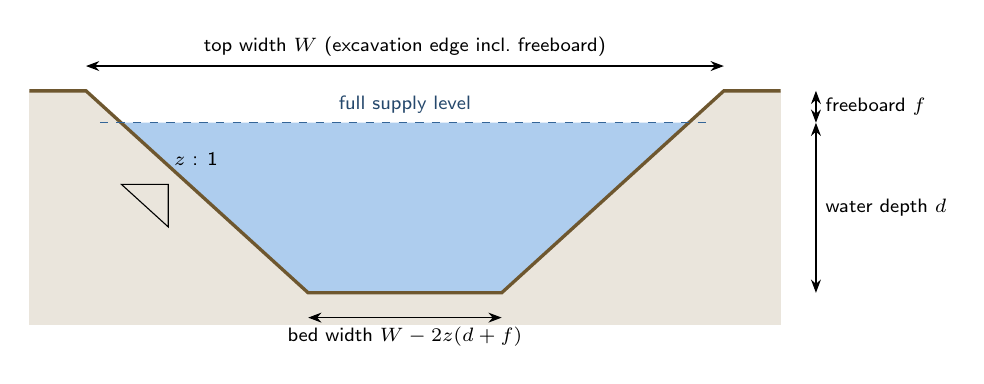
\begin{tikzpicture}[scale=0.9,font=\sffamily\scriptsize]
\def\W{9} \def\d{2.4} \def\z{1.1} \def\f{0.45}
\fill[soil!18] (-0.8,0) -- (\W+0.8,0) -- (\W+0.8,-\d-0.9) -- (-0.8,-\d-0.9) -- cycle;
\fill[white] (0,0) -- (\z*\d+\z*\f,-\d-\f) -- (\W-\z*\d-\z*\f,-\d-\f) -- (\W,0) -- cycle;
\fill[water!45] (\z*\f,-\f) -- (\z*\d+\z*\f,-\d-\f) -- (\W-\z*\d-\z*\f,-\d-\f) -- (\W-\z*\f,-\f) -- cycle;
\draw[soil!80!black,line width=1.2pt] (-0.8,0) -- (0,0) -- (\z*\d+\z*\f,-\d-\f) -- (\W-\z*\d-\z*\f,-\d-\f) -- (\W,0) -- (\W+0.8,0);
\draw[water!70!black,dashed] (\z*\f-0.3,-\f) -- (\W-\z*\f+0.3,-\f);
\node[water!50!black,anchor=south] at (\W/2,-\f) {full supply level};
\draw[{Stealth}-{Stealth}] (0,0.35) -- node[above]{top width $W$ (excavation edge incl.\ freeboard)} (\W,0.35);
\draw[{Stealth}-{Stealth}] (\z*\d+\z*\f,-\d-\f-0.35) -- node[below]{bed width $W-2z(d+f)$} (\W-\z*\d-\z*\f,-\d-\f-0.35);
\draw[{Stealth}-{Stealth}] (\W+1.3,-\f) -- node[right]{water depth $d$} (\W+1.3,-\d-\f);
\draw[{Stealth}-{Stealth}] (\W+1.3,0) -- node[right]{freeboard $f$} (\W+1.3,-\f);
\draw (0.5,-0.55*\d) -- ++(\z*0.6,-0.6) -- ++(0,0.6) -- cycle;
\node at (1.55,-0.4*\d) {$z$ : 1};
\end{tikzpicture}
  \caption{Cross-section of the excavated pond with the design variables.}
  \label{fig:section}
  \Description{Cross-section of a trapezoidal excavated pond in soil. The top width W includes
  the freeboard f above the full supply level; the water depth is d; the side slopes are z to
  1; the bed width is W minus 2 z times d plus f.}
\end{figure}

%% =====================================================================
\section{Implementation}
\label{sec:implementation}
The back end is 3\,515 lines of Python in sixteen modules (Table~\ref{tab:modules}); the front
end is 1\,204 lines of HTML, CSS and JavaScript; the tests are 374 lines. \code{main.py}
handles only HTTP; \code{pipeline.py} orchestrates; each analysis module is a function of
arrays and parameters that can be tested in isolation; network and disk I/O are confined to
\code{tiles.py}, \code{rainfall.py}, \code{landcover.py}, \code{geocode.py} and \code{db.py}.

\begin{table}[h]
  \caption{Back-end modules}
  \label{tab:modules}
  \small
  \begin{tabularx}{\linewidth}{@{}lrY@{}}
    \toprule
    Module & Lines & Responsibility \\
    \midrule
    \code{main.py} & 243 & Routes, validation, error mapping, static front end \\
    \code{schemas.py} & 98 & Pydantic request/response models (drive \code{/docs}) \\
    \code{pipeline.py} & 365 & Orchestration, sea mask, per-candidate evaluation, persistence \\
    \code{tiles.py} & 169 & Web-Mercator maths, parallel tile download with retries, disk cache, mosaic \\
    \code{elevation.py} & 91 & DEM from terrain tiles, Open-Meteo fallback \\
    \code{terrain.py} & 197 & Projection, grid, contour interpolation, slope, curvature \\
    \code{kml\_parser.py} & 225 & KML/KMZ parsing, four elevation-detection strategies \\
    \code{hydrology.py} & 239 & Priority-Flood, D8, accumulation, edge inflow, catchment, boundary \\
    \code{landcover.py} & 501 & OpenCV classification, Overpass client (cache, circuit breaker), rasterisation, tiers \\
    \code{pond.py} & 263 & Site scoring, independent ranking, snapping, natural-basin storage \\
    \code{rainfall.py} & 340 & CHIRPS/Open-Meteo/NASA clients, parallel fetch, cache, scaling, statistics \\
    \code{runoff.py} & 150 & Curve numbers, AMC adjustment, daily SCS-CN, rational method \\
    \code{design.py} & 192 & Frustum geometry, depth selection, losses, footprint \\
    \code{layers.py} & 262 & Contours, drainage network, land polygons, PNG overlays \\
    \code{db.py}, \code{geocode.py} & 180 & SQLite persistence and cache; Nominatim client \\
    \bottomrule
  \end{tabularx}
\end{table}

\subsection{Backend and API Design}
The API is REST over JSON (Table~\ref{tab:api}); the full schema is generated from the
Pydantic models and served at \code{/docs}. One analysis is a single synchronous request that
returns one self-describing document (Listing~\ref{lst:response}), so the client needs no
follow-up calls and a saved result can be re-displayed exactly.

\begin{table}[h]
  \caption{HTTP endpoints}
  \label{tab:api}
  \small
  \begin{tabularx}{\linewidth}{@{}lP{4.6cm}Y@{}}
    \toprule
    Method & Path & Purpose \\
    \midrule
    POST & \code{/api/analyze} & Full analysis of a village location (JSON; only \code{lat}, \code{lon} required) \\
    POST & \code{/analyzeContour} & Full analysis of an uploaded KML/KMZ (multipart); alias \code{/findCatchment} \\
    GET & \code{/api/geocode?q=} & Village search \\
    GET & \code{/api/reverse?lat=\&lon=} & Place name for a map click \\
    GET & \code{/api/rainfall?lat=\&lon=\&years=} & Rainfall statistics only \\
    GET & \code{/api/analyses} & List saved analyses (summaries) \\
    GET / DELETE & \code{/api/analyses/\{id\}} & Retrieve or delete one analysis \\
    GET & \code{/health} & Liveness probe for the hosting platform \\
    GET & \code{/}, \code{/docs} & Front end; interactive API documentation \\
    \bottomrule
  \end{tabularx}
\end{table}

\begin{lstlisting}[caption={Request and abridged response of \texttt{POST /api/analyze} (Hiware Bazar).},label={lst:response},captionpos=b]
POST /api/analyze   {"lat": 19.068, "lon": 74.601, "village": "Hiware Bazar"}

{ "status": "success", "mode": "village", "analysis_id": 22,
  "pond_site":   {"location": {"lat": 19.07995, "lon": 74.59600, "elevation_m": 708.95},
                  "slope_deg": 0.4, "land_tier": "open_land", "reason": "Rank 1: combined score 0.92 ..."},
  "catchment":   {"area_hectares": 137.6, "perimeter_m": 7720, "relief_m": 44.8,
                  "boundary_geojson": {"type": "Feature", "geometry": {"type": "Polygon", ...}}},
  "rainfall":    {"source": "CHIRPS v2.0 daily, 0.05 deg", "period": "2006-2025",
                  "mean_annual_mm": 712.7, "dependable_75pct_mm": 599, "annual_series": [...]},
  "runoff":      {"composite_curve_number": 85.8, "mean_annual_runoff_m3": 134368,
                  "dependable_annual_runoff_m3": 73712},
  "pond_design": {"storage_capacity_m3": 36856, "water_depth_m": 3.0, "top_length_m": 141.3,
                  "top_width_m": 94.2, "excavation_volume_m3": 43604, "notes": [...]},
  "candidates":  [ {"rank": 1, ...}, ..., {"rank": 5, ...} ],
  "layers":      {"contours": {...}, "drainage": {...}, "suitable_land": {...},
                  "elevation_png": "data:image/png;base64,...", "bounds": [...]},
  "warnings": [], "method": {"timings_s": {...}, ...}, "processing_seconds": 38.1 }
\end{lstlisting}

\paragraph{Authentication.} There is none: the system is a single-tenant planning tool over
public data, so every user may run and view analyses (Section~\ref{sec:csd-themes} discusses
what adding it would involve).

\paragraph{Error handling.} All errors share one JSON shape, \code{\{"status":"error",
"detail":"..."\}}. Table~\ref{tab:failures} lists how each failure is handled. The design rule
is: a \emph{required} input that cannot be obtained is an error with a precise message;
\emph{optional} evidence that cannot be obtained degrades the result and is listed in the
response's \code{warnings}.

\begin{table}[h]
  \caption{Failure handling}
  \label{tab:failures}
  \small
  \begin{tabularx}{\linewidth}{@{}P{3.6cm}Y@{}}
    \toprule
    Failure & Behaviour \\
    \midrule
    Invalid input; empty or oversized upload & 422 with field-level message; 400; 413 \\
    Location mostly at sea & 422 ``Choose a location on land'' \\
    Terrain tile download fails & 5 attempts with back-off, then the Open-Meteo elevation fallback; 502 if both fail \\
    Esri imagery missing or placeholder tiles & Land assessment continues on OSM, parcels and slope; warning \\
    Overpass down, rate-limited or firewalled & 5\,s connect timeout; serialised calls; 7-day cache; 2-minute fail-fast cool-down; warning \\
    CHIRPS unavailable & Retries, then Open-Meteo ERA5, then NASA POWER; failures listed in \code{fallback\_errors} \\
    All rainfall sources fail & Rational method on a fallback annual rainfall; warning \\
    No pond fits on the land patch & Pond reported as 0\,m$^3$ with an explanatory note (no crash) \\
    \bottomrule
  \end{tabularx}
\end{table}

\paragraph{Security.} Every request is validated by Pydantic (coordinate ranges, enumerations
such as soil group A--D, numeric bounds), uploads are capped at 25\,MB, and only the server
calls third-party services. No secret is needed to run the system; the optional MapTiler key
lives in an untracked \code{.env} file. Before the repository was made public, its full git
history was scanned for credential files, keys and tokens. CORS is open (\code{*}) because the
API serves only public data; a multi-tenant deployment would restrict it.

\subsection{Frontend and Visualization}
The front end (Figure~\ref{fig:ui}) is a single page with \emph{Village}, \emph{Contour file}
and \emph{History} tabs over a Leaflet map. The Village tab offers search, a preview of the
analysis square, parcel drawing and GeoJSON upload with Leaflet.draw, an optional manual pond
pin and advanced parameters (soil group, rainfall dataset and normal, storage fraction, depth
and slope limits). A staged progress overlay covers the map while an analysis runs. Results
appear as a headline storage card with four key figures; a ranked candidate table mirrored by
numbered map markers (selecting one redraws everything for it); and \emph{Pond},
\emph{Rainfall}, \emph{Runoff} and \emph{Site \& land} sub-tabs with a pond cross-section and
Chart.js charts (Figure~\ref{fig:uiparts}). Layers --- contours, drainage, catchment,
available land, land-cover and relief rasters, pond footprints --- can be toggled. Results
export as JSON or GeoJSON and print through a dedicated stylesheet. Accessibility work includes
ARIA tab semantics, keyboard operation of lists and table rows, visible focus outlines, a skip
link, labelled map and chart regions, reduced-motion support and AA text contrast.

\begin{figure}[h]
  \centering
  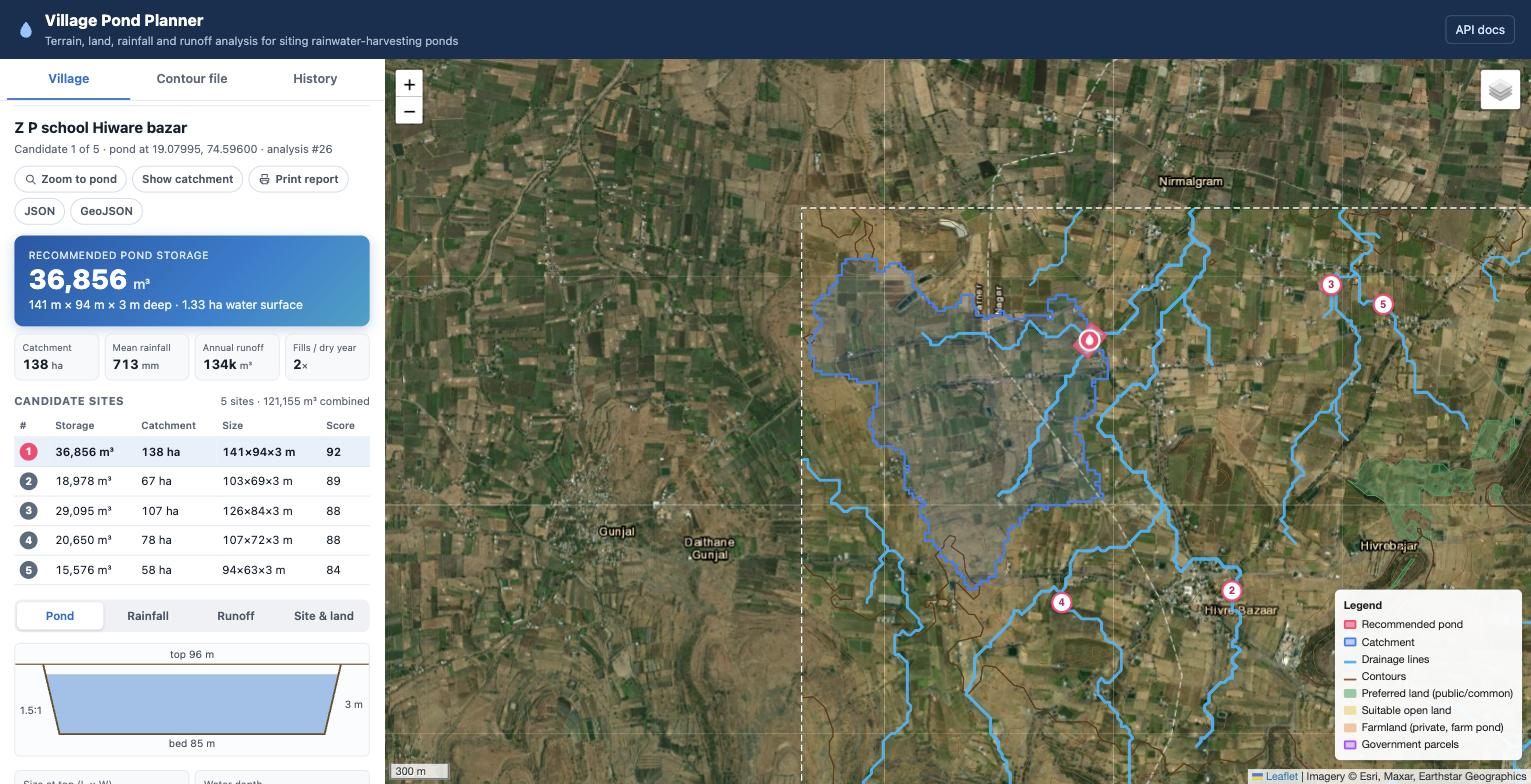
\includegraphics[width=\linewidth]{../docs/app_screenshot.jpg}
  \caption{Application interface showing the results overlay for Hiware Bazar.}
  \label{fig:ui}
  \Description{Screenshot of the web application. A sidebar on the left shows the headline
  pond storage, four key indicators and a ranked table of five candidate sites. The map on the
  right shows satellite imagery with contour lines, the drainage network, the blue catchment
  boundary of candidate 1 and numbered markers for candidates 2 to 5.}
\end{figure}

\begin{figure}[h]
  \centering
  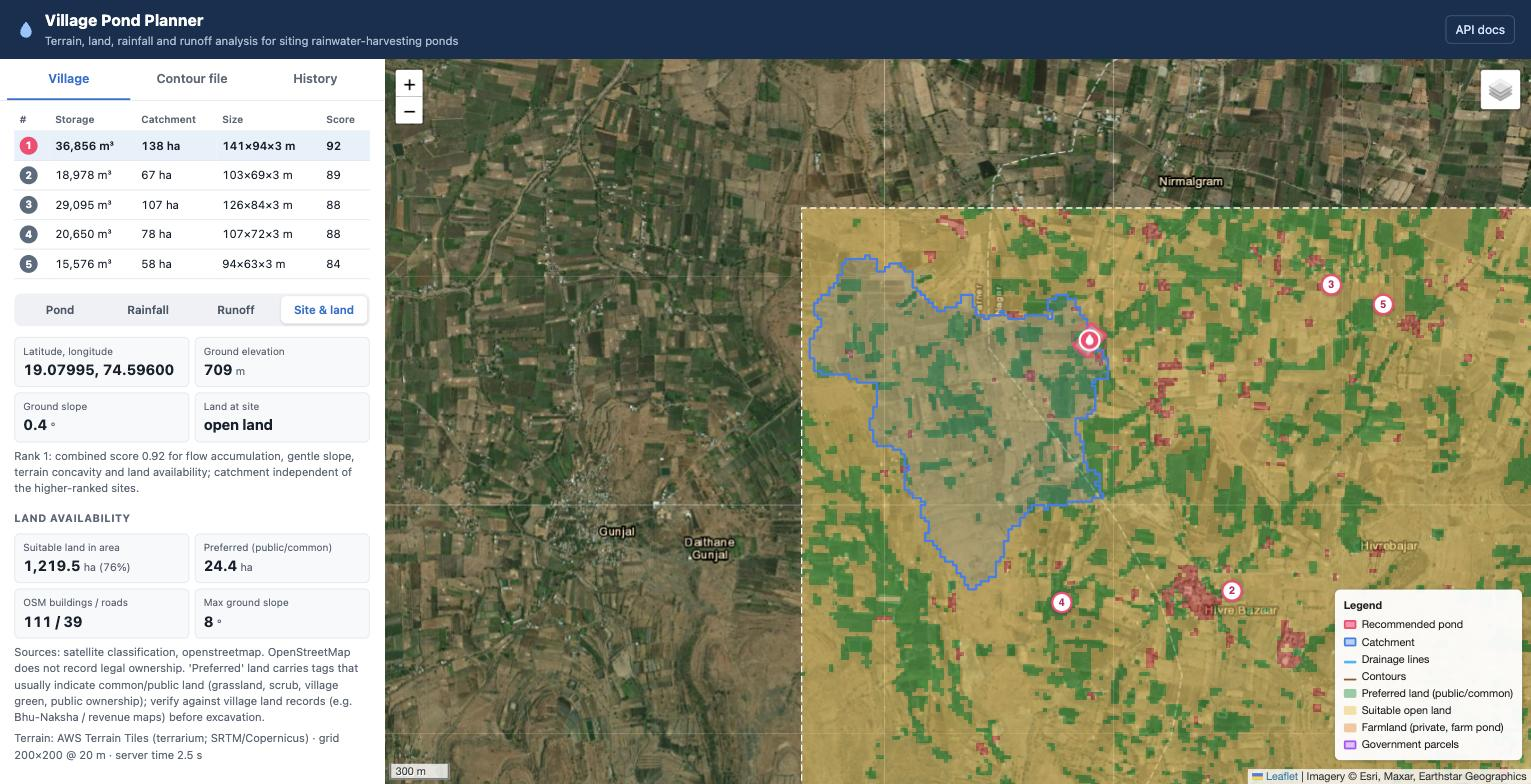
\includegraphics[height=6.2cm]{../docs/landcover_overlay.jpg}\hfill
  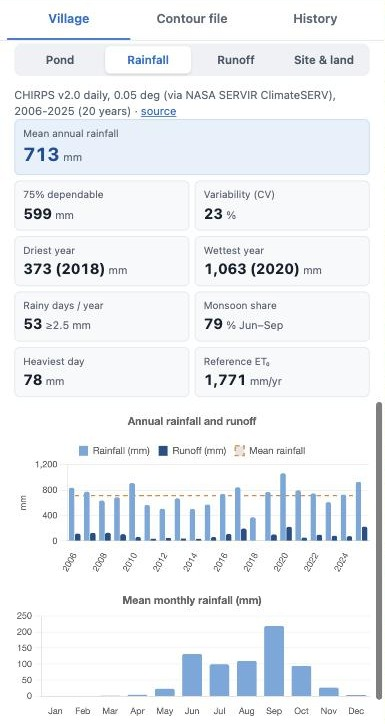
\includegraphics[height=6.2cm]{../docs/rainfall_sidebar.jpg}
  \caption{Further views: (left) land-cover classification overlay --- green vegetation, yellow
  open land, red built-up --- with candidate 1's catchment; (right) the Rainfall tab.}
  \label{fig:uiparts}
  \Description{Left: satellite map tinted by land-cover class, with the village settlement in
  red at lower right and the catchment outline of candidate 1. Right: the rainfall sidebar with
  summary statistics and a bar chart of annual rainfall.}
\end{figure}

\subsection{Database and Storage}
Figure~\ref{fig:schema} shows the schema. \code{analyses} stores every completed analysis
twice: a compact summary for the history list and the full response for exact re-display,
with the village, mode, top-site coordinates and a UTC timestamp; an index on
\code{created\_at} serves the newest-first history query, and single analyses are fetched by
primary key. \code{api\_cache} memoises external responses with a time-to-live
(Table~\ref{tab:cache}). Map tiles are cached as files keyed by source, zoom and tile
coordinates. Spatial results (catchments, footprints, land polygons) are stored as GeoJSON
inside the result document rather than in spatial tables, because they are only ever read
back whole. All access goes through \code{db.py}, which serialises writes with a lock.

\begin{figure}[h]
  \centering
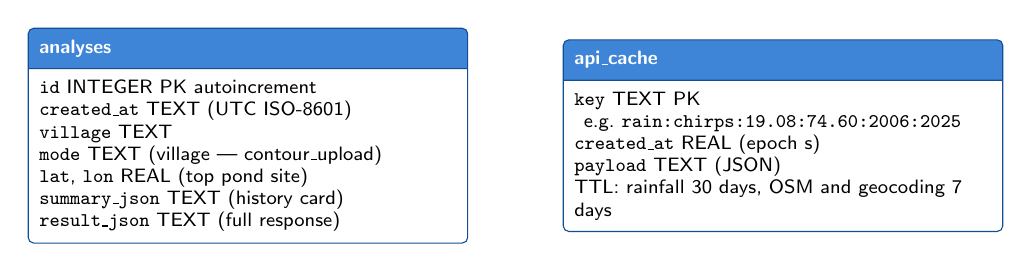
\begin{tikzpicture}[font=\sffamily\scriptsize,
  tbl/.style={rectangle split,rectangle split parts=2,draw=accent!70!black,rounded corners=2pt,
    rectangle split part fill={accent!85,white},align=left,inner sep=4pt,text width=5.3cm}]
\node[tbl] (a) {\textcolor{white}{\textbf{analyses}}
\nodepart{two}\texttt{id} INTEGER PK autoincrement\\ \texttt{created\_at} TEXT (UTC ISO-8601)\\ \texttt{village} TEXT\\ \texttt{mode} TEXT (village | contour\_upload)\\ \texttt{lat}, \texttt{lon} REAL (top pond site)\\ \texttt{summary\_json} TEXT (history card)\\ \texttt{result\_json} TEXT (full response)};
\node[tbl,right=1.2cm of a] (c) {\textcolor{white}{\textbf{api\_cache}}
\nodepart{two}\texttt{key} TEXT PK\\ \phantom{x}e.g.\ \texttt{rain:chirps:19.08:74.60:2006:2025}\\ \texttt{created\_at} REAL (epoch s)\\ \texttt{payload} TEXT (JSON)\\ TTL: rainfall 30 days, OSM and geocoding 7 days};
\end{tikzpicture}
  \caption{SQLite schema. An index on \texttt{analyses(created\_at)} serves the history list.}
  \label{fig:schema}
  \Description{Two tables. analyses: id integer primary key, created\_at text, village text,
  mode text, lat and lon real, summary\_json text, result\_json text. api\_cache: key text
  primary key, created\_at real, payload text, with time-to-live of 30 days for rainfall and 7
  days for geocoding.}
\end{figure}

\begin{table}[h]
  \caption{Cache levels}
  \label{tab:cache}
  \small
  \begin{tabularx}{\linewidth}{@{}P{3.0cm}P{5.2cm}lY@{}}
    \toprule
    What & Key & TTL & Effect \\
    \midrule
    Terrain and imagery tiles & \code{cache/<source>/<z>/<x>/<y>} (files) & none & No re-download of a village's tiles \\
    Rainfall series & \code{rain:<source>:<lat>:<lon>:<y0>:<y1>} (0.01\textdegree) & 30 d & First run 44\,s $\rightarrow$ repeat 1.3\,s \\
    OpenStreetMap features & \code{osm:<bbox to 5 decimals>} & 7 d & Concurrent users stay within Overpass's limit \\
    Geocoding & \code{geo:<country>:<limit>:<query>} & 7 d & Respects Nominatim's 1 request/s policy \\
    Results & \code{analyses} table & kept & History, re-display, export \\
    \bottomrule
  \end{tabularx}
\end{table}

\subsection{Deployment}
\label{sec:deploy}
The application ships with a \code{Dockerfile} (\code{python:3.12-slim}) and a Render
blueprint with a health check. It was also deployed on a college lab machine, which became an
important test environment. Four Ubuntu 24.04 machines (120 cores, 125\,GB RAM each) were
reachable only through forwarded SSH ports; none had Docker, tmux or rsync, and outbound
internet access was unreliable. We inspected all four and deployed on one, chosen because it
reached the most data services: one instance is enough, since the application is CPU-light
and limited by external APIs (Section~\ref{sec:loadtest}), and SQLite favours a single writer.
The project was copied with \code{tar} over SSH, installed into a virtual environment, and
started with \code{nohup setsid uvicorn --host 0.0.0.0} through a small control script
(\code{pond.sh start|stop|restart|status|logs}) so it survives logout. Users reach it through
an SSH tunnel (\code{ssh -L 8080:localhost:8000 sys4}). Measurements on that network are
reported in Section~\ref{sec:defects}.

%% =====================================================================
\section{CSD Themes and Topics Applied in the Project}
\label{sec:csd-themes}
Table~\ref{tab:csd-themes} maps the Computer System Design themes we applied to concrete parts
of the system. Themes we did not implement are discussed after the table.

\begin{table*}[t]
  \caption{Mapping of core CSD themes/topics to their use in this project}
  \label{tab:csd-themes}
  \small
  \begin{tabularx}{\linewidth}{@{}P{2.5cm}P{4.6cm}Y@{}}
    \toprule
    CSD Theme/Topic & Where used in the project & Justification / design rationale \\
    \midrule
    API Design (REST) & \code{/api/analyze}, \code{/analyzeContour}, \code{/api/rainfall}, \code{/api/analyses/\{id\}}; Pydantic schemas; OpenAPI at \code{/docs} & Resources map naturally to REST. One request returns one self-describing document (results, layers, warnings, methods, timings), so the client needs no follow-up calls. The schema is the contract and is validated on every request; errors share one shape. \\
    Caching & Tile files; \code{api\_cache} (rainfall 30\,d, OSM 7\,d, geocoding 7\,d); saved results (Table~\ref{tab:cache}) & External APIs dominate latency and are rate-limited: a cached analysis takes 1.3\,s instead of 44\,s. The OSM cache was added after load testing showed concurrent users exhausting the Overpass quota. \\
    Database Indexing / Query Optimization & Primary keys on \code{analyses.id}, \code{api\_cache.key}; index on \code{analyses(created\_at)}; summary stored apart from the full result & The two hot queries --- newest $n$ analyses, cache lookup by key --- are index scans. The history list reads only the small summary, not multi-megabyte results. No spatial index is needed: no query searches by location. \\
    Concurrency / Asynchronous Processing & Thread pools: 8 parallel tile downloads; two CHIRPS decades in parallel; rainfall and ET$_0$ in parallel; FastAPI's worker pool per request; database write lock; Overpass lock & Work is I/O-bound on slow APIs, so overlapping downloads cuts first-run time. NumPy and OpenCV release the GIL, so 8 concurrent analyses run as fast as one. Serialising Overpass calls respects its per-IP limit. \\
    Microservices vs.\ Monolith & Modular monolith: one FastAPI process, layered modules & One developer, one deployable unit, and stages that exchange 40\,000-cell arrays --- services would add serialisation and network hops for no gain. Module boundaries keep a later split (e.g.\ a rainfall service) possible. \\
    Design Patterns & Pipeline (\code{pipeline.run}); fallback chain of providers (rainfall, elevation); circuit breaker (Overpass cool-down); retry with back-off (tiles, rainfall); data-access module (\code{db.py}); DTOs (Pydantic) & Each stage is replaceable; the fallback chain implements graceful degradation uniformly; the circuit breaker stops one failing service from queueing every request behind a timeout; SQL isolated in one module could move to PostgreSQL. \\
    Containerization / Deployment & \code{Dockerfile}, Render blueprint with health check; lab-server deployment with venv, \code{nohup setsid}, control script, SSH tunnel & Reproducible environment for grading; the health check lets a platform restart a failed instance; the lab deployment works where Docker is not available. \\
    Error Handling and Resilience & Fallbacks for every source; retries; timeouts; warnings; uniform error JSON; input validation; upload cap (Table~\ref{tab:failures}) & Public APIs are rate-limited and sometimes unreachable; the system must degrade, not fail, and say exactly what was degraded. \\
    Algorithms and Complexity & Priority-Flood $O(n\log n)$; vectorised D8 $O(n)$; sorted accumulation; BFS catchment $O(n)$; independent best-first ranking (Table~\ref{tab:algos}) & Terrain analysis of 40\,000 cells takes 60\,ms, negligible next to I/O. Priority-Flood avoids the $O(n^2)$ worst case of iterative pit filling. \\
    Testing Strategy & 30 unit + 5 API tests; validation against independent data; end-to-end, load and deployment tests (Section~\ref{sec:testing}) & Unit tests pin formulas to analytic answers; validation measures real accuracy; system tests found six defects that unit tests missed, each now covered by a regression test where possible. \\
    Version Control & Git; public GitHub repository; history scanned for secrets before publishing & Every change is a reviewable commit with a descriptive message; the public link lets graders inspect the code. \\
    \bottomrule
  \end{tabularx}
\end{table*}

\paragraph{Themes not implemented.} \emph{Load balancing}: one Uvicorn process serves the
expected load; the bottleneck is external APIs, not CPU, and SQLite favours a single writer.
Scaling out would mean several Uvicorn workers behind a reverse proxy such as Nginx, with the
database and caches moved to PostgreSQL and Redis so that instances share them.
\emph{Authentication and authorisation}: all data is public and the tool is single-tenant; a
multi-panchayat deployment would need login (e.g.\ OAuth) and per-village ownership of saved
analyses. \emph{CI/CD}: there is no pipeline yet; running the 35 tests in GitHub Actions on every
push is the obvious next step and would have caught the broken file described in
Section~\ref{sec:defects} automatically.

\paragraph{Deep dive 1: caching and resilience around external APIs.} Every slow or fragile
dependency sits behind a cache and a fallback. Load testing showed why both are needed
(Section~\ref{sec:loadtest}): with four concurrent analyses, uncached OpenStreetMap queries
exceeded Overpass's per-IP limit, each request waited about 44\,s and then silently lost all
its OSM exclusions. Adding a cache and a lock alone made things worse when Overpass was down
--- requests queued behind one another's timeouts, up to 293\,s. Only the third step, a
circuit breaker that fails fast for two minutes after a failure, gave the intended behaviour:
one timeout per outage instead of one per request.

\paragraph{Deep dive 2: a modular monolith instead of microservices.} The stages pass large
NumPy arrays between them, the team is one person, and the hosting is a single instance. A
monolith with strict module boundaries --- pure functions of arrays, I/O confined to five
modules --- gives the testability of services without their operational cost: one process to
deploy, monitor and restart, and no network serialisation between stages.

\paragraph{Deep dive 3: choosing data by measurement.} The rainfall source was initially
Open-Meteo with NASA POWER as fallback. Validation against IMD normals showed errors up to
92\,\% in exactly the rain-shadow areas where ponds matter most, so CHIRPS became the default
and the others fallbacks --- an architectural decision driven by data quality rather than
convenience.

%% =====================================================================
\section{Results and Evaluation}
\label{sec:results}

\subsection{Case Study: Hiware Bazar}
Hiware Bazar (Ahilyanagar district, Maharashtra) is a model watershed village on the
semi-arid Deccan plateau. We analysed a 4\,km$\times$4\,km area centred at
19.068\textdegree{}N, 74.601\textdegree{}E with soil group C and default parameters. The
figures are from a run on 27 September 2026; because imagery, OpenStreetMap and CHIRPS are live
sources, later runs can differ slightly (a rerun on 2 October, after one road was removed from
OpenStreetMap, swapped the two nearly equal leading sites).

The DEM spans 692--875\,m. OpenStreetMap supplied 111 buildings, 39 roads and 23 water
features; after all exclusions 76\,\% of the area (1\,219\,ha) is suitable for excavation, of
which 24.4\,ha carries common-land tags. CHIRPS gives a mean annual rainfall of 713\,mm for
2006--2025, a 75\,\%-dependable rainfall of 599\,mm and a coefficient of variation of 23\,\%
(373\,mm in 2018 to 1\,063\,mm in 2020); 79\,\% falls in June--September, over 53 rainy days a
year. Reference ET$_0$ is 1\,771\,mm/yr, 1\,249\,mm of it in the dry season. The ranking
algorithm found five independent sites, all on open land with slopes of 0.1--1.6\textdegree{}
(Table~\ref{tab:cands}, Figure~\ref{fig:results}).

\begin{table}[h]
  \caption{Ranked candidate ponds for Hiware Bazar (soil group C, CHIRPS 2006--2025)}
  \label{tab:cands}
  \small
  \begin{tabular}{@{}cccrrrrc@{}}
    \toprule
    Rank & Score & Location (\textdegree N, \textdegree E) & Catchment & Mean runoff & Dep.\ runoff & Storage & Top size \\
     & & & (ha) & (m$^3$/yr) & (m$^3$/yr) & (m$^3$) & (m) \\
    \midrule
    1 & 0.92 & 19.07995, 74.59600 & 137.6 & 134\,368 & 73\,712 & 36\,856 & 141$\times$94 \\
    2 & 0.89 & 19.06862, 74.60285 & 67.3 & 68\,007 & 37\,955 & 18\,978 & 103$\times$69 \\
    3 & 0.88 & 19.08247, 74.60760 & 106.5 & 105\,393 & 58\,190 & 29\,095 & 126$\times$84 \\
    4 & 0.88 & 19.06808, 74.59466 & 78.5 & 75\,657 & 41\,301 & 20\,650 & 107$\times$72 \\
    5 & 0.84 & 19.08157, 74.61008 & 57.7 & 56\,694 & 31\,153 & 15\,576 & 94$\times$63 \\
    \midrule
    \multicolumn{3}{@{}l}{\textbf{Total}} & \textbf{447.6} & \textbf{440\,119} & & \textbf{121\,155} & \\
    \bottomrule
  \end{tabular}
\end{table}

\begin{figure}[h]
  \centering
  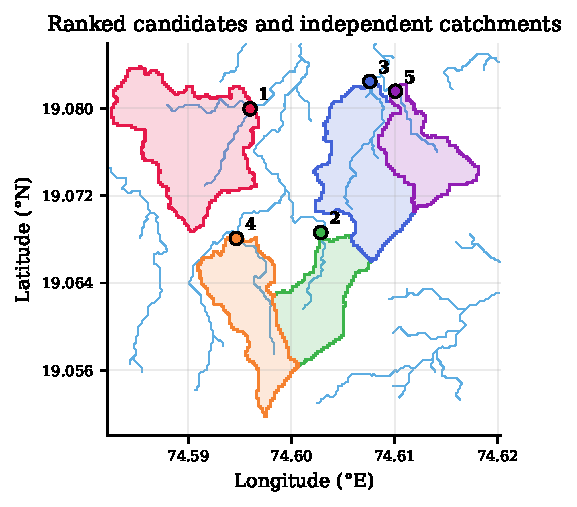
\includegraphics[width=0.62\linewidth]{figures/candidates.pdf}\\[4pt]
  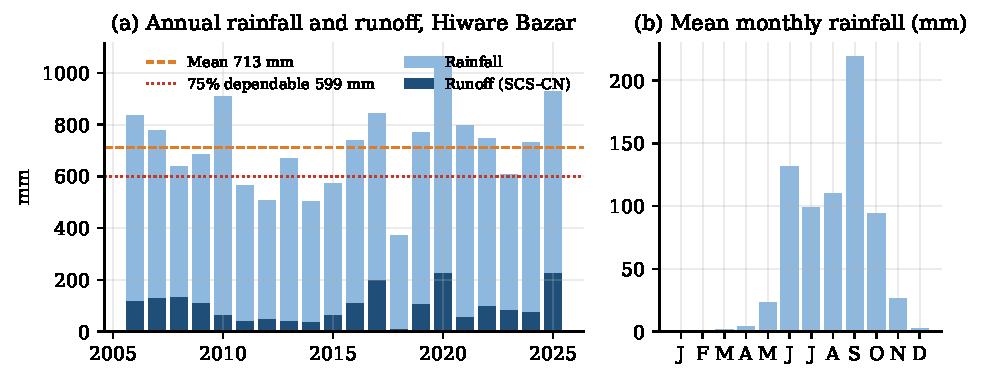
\includegraphics[width=\linewidth]{figures/case_rainfall.pdf}
  \caption{Example results for Hiware Bazar: (top) the five ranked sites and their
  independent catchments; (bottom) annual rainfall and simulated runoff depth 2006--2025, and
  the monthly rainfall climatology.}
  \label{fig:results}
  \Description{Top: map of the analysis area with five numbered pond sites, each surrounded by
  its own catchment outline; the catchments do not overlap. Bottom left: bar chart of annual
  rainfall from 2006 to 2025, ranging from about 370 to 1060 millimetres, with the much
  smaller annual runoff depth overlaid. Bottom right: monthly rainfall, concentrated in June
  to September.}
\end{figure}

The recommended pond (rank 1) lies on open land at 709\,m with a 0.4\textdegree{} slope, at the
outlet of a 137.6\,ha catchment (perimeter 7.72\,km, relief 44.8\,m, mean slope
3.3\textdegree). The catchment is 77\,\% open or fallow land, 22\,\% crops and 1\,\% built-up
(composite CN 85.8), giving a mean runoff of 98\,mm/yr --- an effective runoff coefficient of
0.14 --- or 134\,368\,m$^3$/yr, and 73\,712\,m$^3$ in a dependable year. Table~\ref{tab:design}
gives the design. Dry-season evaporation removes about 44\,\% of the storage, which is
realistic for the Deccan and is why the design prefers depth to area once land is limited.
Together the five ponds capture about 28\,\% of the mean runoff of their catchments, leaving
most of the flow to downstream users.

\begin{table}[h]
  \caption{Recommended pond, rank 1}
  \label{tab:design}
  \small
  \begin{tabular}{@{}ll@{\hspace{2.5em}}ll@{}}
    \toprule
    Storage capacity & \textbf{36\,856\,m$^3$} & Water spread area & 1.33\,ha \\
    Top size (L$\times$W) & 141.3\,m$\times$94.2\,m & Excavation volume & 43\,604\,m$^3$ \\
    Bed size (L$\times$W) & 132.3\,m$\times$85.2\,m & Dry-season evaporation & 16\,099\,m$^3$ (44\,\%) \\
    Water depth + freeboard & 3.0\,m + 0.5\,m & Seepage (4 months) & 3\,384\,m$^3$ \\
    Side slope & 1.5\,:\,1 & Fills per dependable year & 2.0 \\
    \bottomrule
  \end{tabular}
\end{table}

\subsection{Validation Against Reference Data}
Each component was checked against independent references.

\paragraph{Rainfall.} For six IMD observatories in contrasting climates, each dataset's
1991--2020 mean annual rainfall was compared with the IMD normal (Table~\ref{tab:valrain},
Figure~\ref{fig:valrain}). CHIRPS has a mean absolute error of 8.9\,\%; NASA POWER 26.1\,\%,
with $+92\,\%$ at Pune, where its $\sim$50\,km cells mix the wet windward Ghats with the dry
plateau. CHIRPS underestimates the desert ($-28\,\%$ at Jaisalmer), a known weakness of
satellite rainfall in arid regions.

\begin{table}[h]
  \caption{Mean annual rainfall 1991--2020 (mm) and error relative to the IMD normal}
  \label{tab:valrain}
  \small
  \begin{tabular}{@{}llrrrrr@{}}
    \toprule
    Station & Climate & IMD & CHIRPS & Error & NASA POWER & Error \\
    \midrule
    Ahmednagar & semi-arid, rain shadow & 608.1 & 658.1 & +8.2\,\% & 652.0 & +7.2\,\% \\
    Pune & leeward Western Ghats & 841.2 & 897.9 & +6.7\,\% & 1616.7 & \textbf{+92.2\,\%} \\
    Jaisalmer & arid & 256.9 & 184.8 & $-$28.1\,\% & 210.1 & $-$18.2\,\% \\
    Bengaluru & semi-arid plateau & 1077.8 & 1054.0 & $-$2.2\,\% & 858.7 & $-$20.3\,\% \\
    Chennai & NE-monsoon coast & 1408.4 & 1396.8 & $-$0.8\,\% & 1237.9 & $-$12.1\,\% \\
    Mumbai & windward coast & 2502.3 & 2684.6 & +7.3\,\% & 2341.7 & $-$6.4\,\% \\
    \midrule
    \multicolumn{2}{@{}l}{Mean absolute error} & & & \textbf{8.9\,\%} & & \textbf{26.1\,\%} \\
    \bottomrule
  \end{tabular}
\end{table}

\begin{figure}[h]
  \centering
  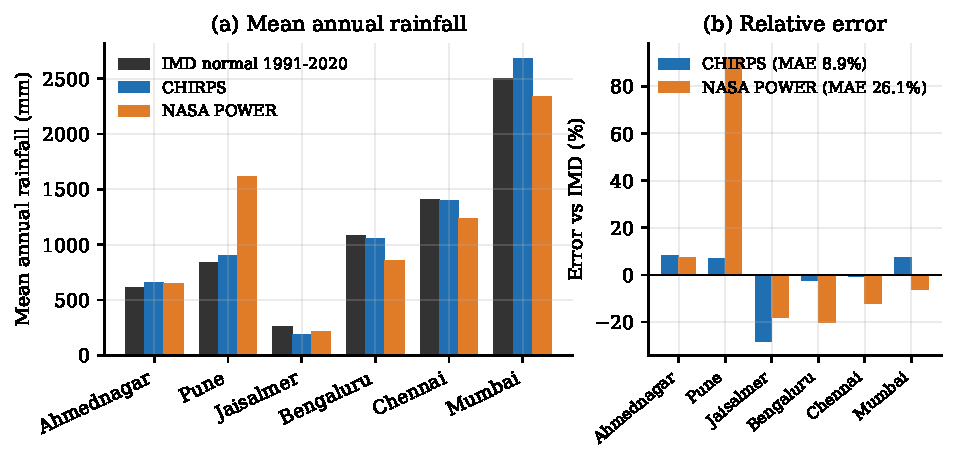
\includegraphics[width=\linewidth]{figures/rainfall_validation.pdf}
  \caption{Rainfall datasets compared with IMD 1991--2020 station normals: (a) mean annual
  rainfall; (b) relative error.}
  \label{fig:valrain}
  \Description{Grouped bar chart of mean annual rainfall at six stations for the IMD normal,
  CHIRPS and NASA POWER, and a second chart of percentage errors, where NASA POWER's Pune bar
  stands out at about plus 92 percent.}
\end{figure}

\paragraph{Elevation.} Terrain-tile elevations at 44 OpenStreetMap summits with surveyed
heights in three regions have a median absolute error of 20\,m and a bias of $-27$\,m
(Figure~\ref{fig:valdem}). Summits are a worst case, since a 30\,m DEM averages a sharp peak
with its flanks; pond sites lie on gentle valley floors and depend on relative elevation.

\paragraph{Land cover.} In four landscapes (semi-arid Maharashtra, irrigated Punjab, wet
Kerala, arid Rajasthan), 25 of the classifier's 20\,m cells each were drawn at random (seed 42),
rendered as 100\,m zoom-18 image chips without the prediction, and labelled by eye; 13 mixed
cells were excluded. Accuracy on the 87 remaining cells is 92\,\%, $\kappa=0.85$
(Figure~\ref{fig:valland}): Hiware Bazar 95\,\%, Ludhiana 100\,\%, Kuttanad 91\,\%, Jaipur
rural 83\,\%. Errors are pale sparse grass called vegetation and half-tree cells. The sample
contained only two built-up cells and no water cells, so those classes are not validated; OSM
is the primary exclusion for both.

\begin{figure}[h]
  \centering
  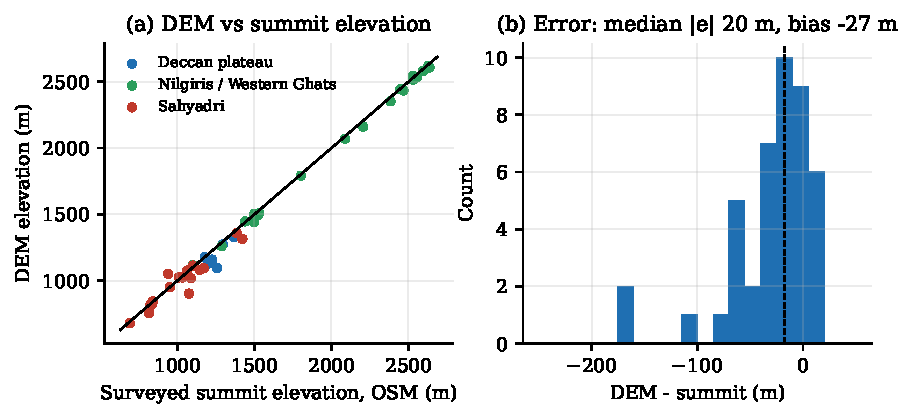
\includegraphics[width=0.56\linewidth]{figures/dem_validation.pdf}\hfill
  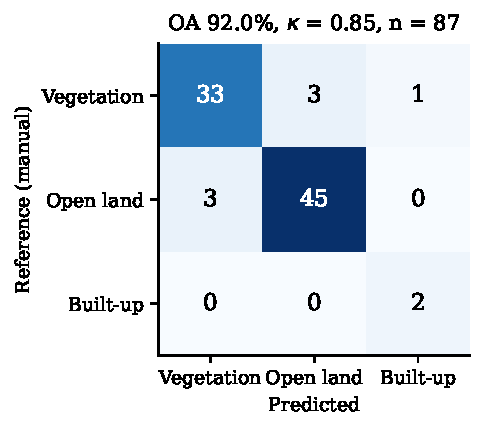
\includegraphics[width=0.40\linewidth]{figures/landcover_confusion.pdf}
  \caption{(left) DEM against surveyed summit elevations; (right) land-cover confusion matrix
  on 87 blind-labelled cells.}
  \label{fig:valdem}
  \label{fig:valland}
  \Description{Left: scatter of DEM elevation against surveyed summit elevation along the 1:1
  line with a histogram of errors centred around minus 20 to minus 30 metres. Right: confusion
  matrix for vegetation, open land, built-up and water, with most counts on the diagonal.}
\end{figure}

\paragraph{Runoff and sensitivity.} Runoff could not be compared with measured flow: no gauged
village-scale catchments exist in open data. The effective coefficient of 0.14 is plausible
for a semi-arid catchment but unverified. The sensitivity analysis (Figure~\ref{fig:sens})
shows an elasticity of about three with respect to rainfall ($\pm10\,\%$ rain gives $-30\,\%$
/ $+31\,\%$ runoff, where the rational method would give $\pm10\,\%$), and a factor of 4.7
between soil groups A and D. Rainfall and soil group therefore dominate the uncertainty in
pond sizing --- which is why the rainfall source was validated and made correctable, and the
soil group is exposed with plain descriptions.

\begin{figure}[h]
  \centering
  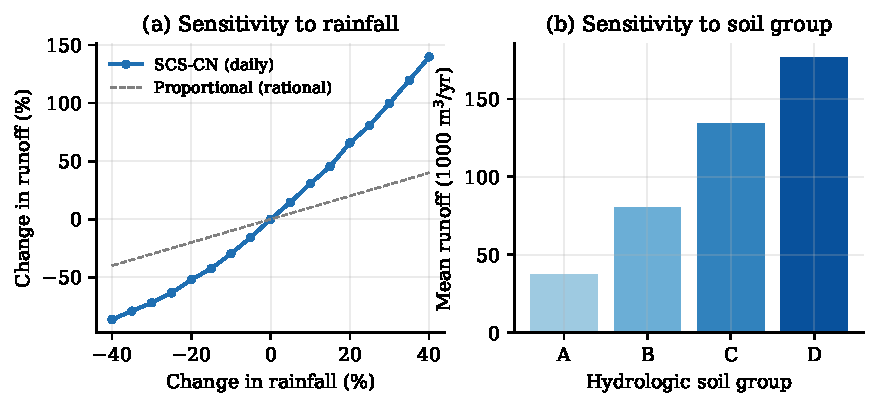
\includegraphics[width=0.92\linewidth]{figures/sensitivity.pdf}
  \caption{Sensitivity of mean annual runoff at Hiware Bazar (rank 1): (a) to a uniform scaling
  of daily rainfall; (b) to hydrologic soil group.}
  \label{fig:sens}
  \Description{Left: runoff rising steeply and non-linearly as rainfall is scaled from 80 to 120
  percent. Right: runoff for soil groups A to D increasing from about 37 thousand to 177
  thousand cubic metres per year.}
\end{figure}

\subsection{Testing Strategy}
\label{sec:testing}
Testing is layered (Table~\ref{tab:tests}). Unit tests pin formulas and the hydrology core to
hand calculations and exact analytic answers --- most notably a synthetic V-valley whose
catchment is known cell for cell. API tests start the real application in-process and check
routing, validation and error shapes without network access. System tests drive the running
server over HTTP with real data, and load tests drive it concurrently.

\begin{table}[h]
  \caption{Test levels}
  \label{tab:tests}
  \small
  \begin{tabularx}{\linewidth}{@{}P{2.4cm}rY@{}}
    \toprule
    Level & Tests & What it checks \\
    \midrule
    Unit: formulas & 19 & SCS runoff (hand-calculated 50.54\,mm case and four more), AMC conversion, runoff volume, frustum volume, width solver, pond rules (incl.\ no-fit), FAO-56 radiation example, rainfall statistics \\
    Unit: hydrology & 5 & No sinks after filling; analytic V-valley catchment; polygon area = cell count; bowl drainage; edge-inflow flag \\
    Unit: siting & 4 & No site in the sea, even in the terrain-only fallback; sea mask keeps an inland polder \\
    Unit: OSM client & 2 & Second query served from cache; failure starts the fail-fast cool-down \\
    API & 5 & App imports and starts; front end and OpenAPI served; error shapes for 422, 400, 404 \\
    System (end to end) & 10 & Health, geocoding, rainfall, cached and new villages, manual pin, contour upload, ocean and bad-input rejection, history --- on the lab server \\
    Load & 5 & 1--16 concurrent analyses; 50 concurrent health checks \\
    Validation & 3 studies & Rainfall (6 stations), elevation (44 summits), land cover (100 cells) \\
    \bottomrule
  \end{tabularx}
\end{table}

\subsection{Defects Found by System Testing}
\label{sec:defects}
All unit tests passed from the start, yet system testing, load testing and the lab deployment
found six defects (Table~\ref{tab:defects}). Each was fixed, and five now have regression tests.

\begin{table*}[t]
  \caption{Defects found after the unit tests passed, and their fixes}
  \label{tab:defects}
  \small
  \begin{tabularx}{\linewidth}{@{}cP{3.0cm}P{3.4cm}YP{2.0cm}@{}}
    \toprule
    \# & Found by & Symptom & Cause and fix & Regression test \\
    \midrule
    1 & End-to-end probe of unusual inputs & A pond 4\,288\,m below sea level in the Pacific; 3 of 5 coastal Konkan sites offshore & The RGB water rule misses teal, turbid water, and Esri serves grey placeholders over the ocean. Fix: DEM-based sea mask (connected low areas with sea-surface or bathymetry seeds), 422 for mostly-sea areas, placeholder detection & 4 tests \\
    2 & Load test, 4 concurrent analyses & 45\,s per request instead of 1.3\,s; all results silently lacked OSM exclusions & Overpass admits $\sim$2 queries per IP; OSM was not cached. Fix: 7-day cache, serialised calls, 2-minute circuit breaker & 2 tests \\
    3 & Lab deployment & Analyses hung for 70\,s or more on ``finding the terrain'' & The campus firewall silently drops Overpass connections (\code{SYN-SENT}); each of two servers waited the full 35\,s read timeout. Fix: 5\,s connect timeout & --- (network) \\
    4 & Lab deployment & ``No elevation source available'' for new villages & DNS failed 2 times in 10; one failed tile of $\sim$30 aborted the analysis and the 3 retries had no pause. Fix: 5 attempts with back-off & --- (network) \\
    5 & Lab deployment (Hyderabad) & HTTP 500, \code{ZeroDivisionError} & In a dense city a land patch can be smaller than the smallest pond; storage was capped to 0 and divided by. Fix: report ``no pond fits here'' & 1 test \\
    6 & Code comparison between laptop and server & App would not start from the laptop copy & An accidental edit left a syntax error in \code{main.py}; no unit test imported it. Fix: restored file; added API tests that import and start the app & 5 tests \\
    \bottomrule
  \end{tabularx}
\end{table*}

The lesson is that a geospatial web application's hardest failures are at its boundaries ---
unusual places on Earth, other people's servers, and real networks --- which only system-level
testing exercises.

\subsection{Performance}
\label{sec:perf}
Laptop timings were measured through the HTTP API on an Apple M4 (10 cores), 2--4 October
2026; server timings on the lab machine (Ubuntu 24.04, 120 cores) on 5 October
(Table~\ref{tab:perf}). Figure~\ref{fig:stages} breaks a cached analysis into stages.

\begin{table}[h]
  \caption{Measured response times}
  \label{tab:perf}
  \small
  \begin{tabularx}{\linewidth}{@{}Yrr@{}}
    \toprule
    Operation & Laptop & Lab server \\
    \midrule
    Village analysis, first run (20 years of CHIRPS downloaded) & 44.2\,s & 59--317\,s$^\ast$ \\
    Village analysis, cached (Hiware Bazar) & 1.3\,s & 3.3\,s \\
    Contour-map analysis (\code{sample\_contours.kml}), first run & 64.6\,s & 171\,s$^\ast$ \\
    \code{GET /api/rainfall}, cached & 8\,ms & --- \\
    \code{GET /api/geocode}, cached & 1\,ms & --- \\
    \code{GET /health}, 50 concurrent & median 2.4\,ms, p95 3.3\,ms & 5\,ms \\
    Test suite (35 tests) & 0.4\,s & 4.0\,s \\
    \bottomrule
  \end{tabularx}\\[2pt]
  {\footnotesize $^\ast$Dominated by the unreliable campus network: timeouts on unreachable
  services before falling back.}
\end{table}

\begin{figure}[h]
  \centering
  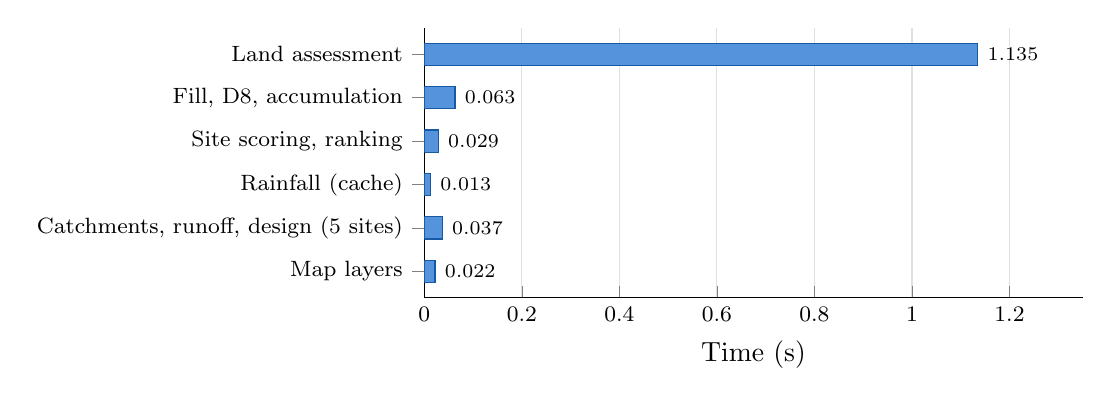
\begin{tikzpicture}
    \begin{axis}[xbar, width=0.82\linewidth, height=5.0cm, xmin=0, xmax=1.35,
      xlabel={Time (s)}, symbolic y coords={Map layers,{Catchments, runoff, design (5 sites)},{Rainfall (cache)},{Site scoring, ranking},{Fill, D8, accumulation},{Land assessment}},
      ytick=data, yticklabel style={font=\footnotesize}, xticklabel style={font=\footnotesize},
      nodes near coords, nodes near coords align={horizontal},
      every node near coord/.append style={font=\scriptsize, /pgf/number format/fixed, /pgf/number format/precision=3},
      bar width=8pt, enlarge y limits=0.12, axis x line*=bottom, axis y line*=left,
      xmajorgrids, grid style={black!12}]
      \addplot[fill=accent!75, draw=accent!80!black] coordinates {
        (0.022,Map layers) (0.037,{Catchments, runoff, design (5 sites)}) (0.013,{Rainfall (cache)})
        (0.029,{Site scoring, ranking}) (0.063,{Fill, D8, accumulation}) (1.135,{Land assessment})};
    \end{axis}
  \end{tikzpicture}
  \caption{Stage times of a cached village analysis (total 1.30\,s). Land assessment ---
  downloading and classifying imagery --- dominates; the hydrology on 40\,000 cells takes
  63\,ms.}
  \label{fig:stages}
  \Description{Horizontal bar chart. Land assessment takes 1.135 seconds; fill, D8 and
  accumulation 0.063; site scoring 0.029; rainfall from cache 0.013; catchments, runoff and
  design for five sites 0.037; map layers 0.022.}
\end{figure}

A first analysis is dominated by the rainfall download (about 35\,s for two parallel ten-year
CHIRPS requests). The computation itself is fast: D8 is vectorised and accumulation is a single
sorted pass.

\subsection{Behaviour Under Load}
\label{sec:loadtest}
Concurrent cached analyses of the same village were sent to one server instance in three
versions of the code (Figure~\ref{fig:load}, Table~\ref{tab:load}). In the baseline, Overpass's
per-IP limit was exceeded: requests beyond the first two waited about 44\,s and lost their
OpenStreetMap data. Caching and serialising Overpass calls alone made the failure case worse:
Overpass had meanwhile started refusing our network (a temporary block, most likely triggered
by the load test), every query failed, nothing was cached, and requests queued behind each
other's timeouts --- up to 293\,s. With the circuit breaker, a batch of four shared a single
36\,s timeout and the next eight requests completed in 1.3\,s each, with the missing OSM data
reported in their warnings. Because NumPy and OpenCV release Python's global interpreter lock,
eight concurrent analyses took no longer than one: CPU is not the bottleneck, external APIs
are. The successful-cache path is covered by unit tests but could not be load-tested live while
Overpass blocked our network.

\begin{table}[h]
  \caption{Concurrent cached analyses: latency (s) by code version}
  \label{tab:load}
  \small
  \begin{tabular}{@{}lccc@{}}
    \toprule
    Code version & 1 request & 4 concurrent (median / max) & 8 concurrent (median / max) \\
    \midrule
    Baseline (no OSM cache) & 1.37 & 45.15 / 45.31 & 2.27 / 44.39 \\
    + cache and serialised calls (Overpass down) & 36.26 & 71.99 / 144.00 & 144.07 / 293.62 \\
    + circuit breaker (Overpass down) & --- & 36.50 / 36.53 & \textbf{1.32 / 1.35} \\
    \bottomrule
  \end{tabular}
\end{table}

\begin{figure}[h]
  \centering
  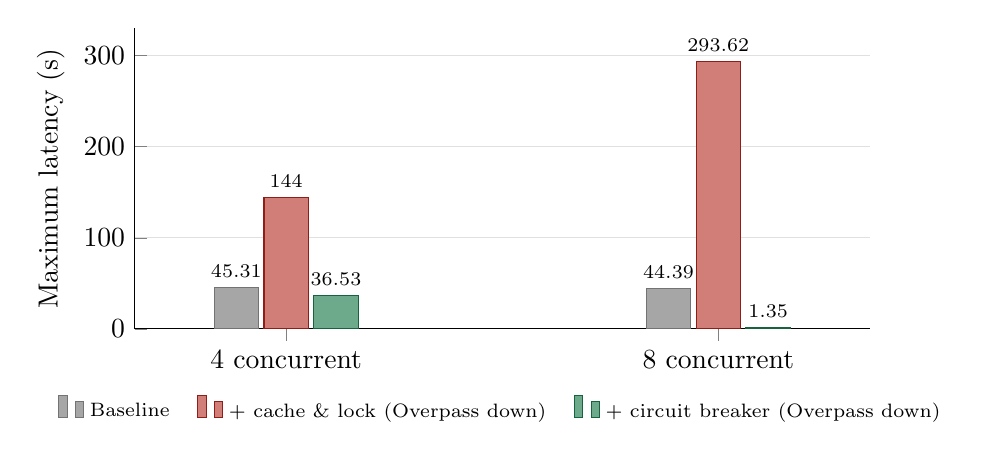
\begin{tikzpicture}
    \begin{axis}[ybar, width=0.9\linewidth, height=5.4cm, ymin=0, ymax=330,
      ylabel={Maximum latency (s)}, symbolic x coords={4 concurrent, 8 concurrent},
      xtick=data, enlarge x limits=0.35, bar width=16pt,
      legend style={font=\scriptsize, at={(0.5,-0.2)}, anchor=north, draw=none, legend columns=-1, /tikz/every even column/.append style={column sep=8pt}},
      nodes near coords, every node near coord/.append style={font=\scriptsize, /pgf/number format/fixed},
      ymajorgrids, grid style={black!12}, axis x line*=bottom, axis y line*=left]
      \addplot[fill=black!35, draw=black!55] coordinates {(4 concurrent,45.31) (8 concurrent,44.39)};
      \addplot[fill=bad!60, draw=bad!80!black] coordinates {(4 concurrent,144.00) (8 concurrent,293.62)};
      \addplot[fill=good!65, draw=good!80!black] coordinates {(4 concurrent,36.53) (8 concurrent,1.35)};
      \legend{Baseline, + cache \& lock (Overpass down), + circuit breaker (Overpass down)}
    \end{axis}
  \end{tikzpicture}
  \caption{Worst-case latency of concurrent cached analyses in three code versions. The circuit
  breaker turns one timeout per request into one timeout per outage.}
  \label{fig:load}
  \Description{Grouped bar chart. For 4 concurrent requests the maximum latency is 45.3 s for the
  baseline, 144 s with cache and lock, and 36.5 s with the circuit breaker. For 8 concurrent
  requests it is 44.4 s, 293.6 s and 1.35 s respectively.}
\end{figure}

%% =====================================================================
\section{Discussion and Limitations}
\label{sec:discussion}
\paragraph{What worked well.} Building everything on one in-memory DEM made the two input
modes share all downstream code. Validating data sources early changed the design for the
better (the switch to CHIRPS). Returning methods, timings and warnings with every result made
failures visible instead of silent. Testing beyond unit tests --- odd locations, concurrency,
a real deployment --- found every serious defect.

\paragraph{What did not.} The RGB water rule (blue brighter than red and green) does not
recognise the turbid, green-tinted water typical of Indian coasts and reservoirs; sea is now
excluded using elevation, but inland water still relies on OpenStreetMap. Dependence on live
public services makes results drift as those services change, and some rate-limit or block
aggressively; on the campus network, analyses often run without OpenStreetMap or imagery, which
degrades siting (a contour analysis returned a 409\,ha catchment instead of 5.4\,ha because a
river was no longer excluded). Results always state this in their warnings, but a planner can
still overlook it.

\paragraph{Data quality and assumptions.} The $\sim$30\,m DEM cannot resolve field bunds,
drains or road embankments, which can redirect flow on the ground. CHIRPS underestimates
deserts ($-28\,\%$ at Jaisalmer). Soil group is a user input and, after rainfall, the most
influential parameter. TR-55 curve numbers were developed for US catchments; their use in India
is standard in watershed manuals but not locally calibrated. Land ownership is inferred, never
certain, and groundwater depth and rock are ignored when choosing depth. All recommendations
therefore need field verification.

\paragraph{Future work.} Sentinel-2 bands (NDWI, NDBI) for water and built-up detection;
ISRIC SoilGrids for automatic soil groups; IMD gridded rainfall as a source; cost per cubic
metre of storage to rank candidates; and a GitHub Actions pipeline running the test suite on
every push.

%% =====================================================================
\section{AI Tool Usage Declaration}
\label{sec:ai-usage}
\todo{List every AI tool you used while developing the project (e.g.\ ChatGPT, Claude, Gemini,
GitHub Copilot) and what you used each for. The paragraph below covers only the final review,
deployment and reporting sessions.}

Claude Code (Anthropic, model Claude Opus 5.5) was used in the final stage of the project for:
reviewing the code and running the application end to end; finding and fixing the six defects
in Table~\ref{tab:defects} and writing their regression tests; load testing and measuring the
performance figures in Section~\ref{sec:perf}; deploying the application on the college lab
server; publishing the repository to GitHub after scanning its history for secrets; updating
the README, validation notes and the main report; and writing this report in the ACM template
from the existing technical report and the measurements above. \todo{Confirm honestly: ``All
AI-assisted code and text was reviewed, understood and, where needed, modified by me before
submission.''}

%% =====================================================================
\begin{thebibliography}{10}
\bibitem{amritsarovar} Ministry of Rural Development, Government of India. 2022. \emph{Mission Amrit Sarovar: Guidelines}.
\bibitem{barnes2014} R. Barnes, C. Lehman, and D. Mulla. 2014. Priority-flood: An optimal depression-filling and watershed-labeling algorithm for digital elevation models. \emph{Computers \& Geosciences} 62, 117--127.
\bibitem{ocallaghan1984} J.~F. O'Callaghan and D.~M. Mark. 1984. The extraction of drainage networks from digital elevation data. \emph{Computer Vision, Graphics, and Image Processing} 28, 3, 323--344.
\bibitem{otsu1979} N. Otsu. 1979. A threshold selection method from gray-level histograms. \emph{IEEE Transactions on Systems, Man, and Cybernetics} 9, 1, 62--66.
\bibitem{funk2015} C. Funk et al. 2015. The climate hazards infrared precipitation with stations --- a new environmental record for monitoring extremes. \emph{Scientific Data} 2, 150066.
\bibitem{hersbach2020} H. Hersbach et al. 2020. The ERA5 global reanalysis. \emph{Quarterly Journal of the Royal Meteorological Society} 146, 730, 1999--2049.
\bibitem{allen1998} R.~G. Allen, L.~S. Pereira, D. Raes, and M. Smith. 1998. \emph{Crop Evapotranspiration: Guidelines for Computing Crop Water Requirements}. FAO Irrigation and Drainage Paper 56, Rome.
\bibitem{tr55} USDA Soil Conservation Service. 1986. \emph{Urban Hydrology for Small Watersheds}. Technical Release 55, 2nd ed.
\bibitem{hawkins1985} R.~H. Hawkins, A.~T. Hjelmfelt, and A.~W. Zevenbergen. 1985. Runoff probability, storm depth, and curve numbers. \emph{Journal of Irrigation and Drainage Engineering} 111, 4, 330--340.
\end{thebibliography}

%% =====================================================================
\appendix

\section{Source Code and Repository}
\label{app:repo}
Repository (public): \url{https://github.com/amandeeip01/village-pond-planner}

\begingroup\raggedright
\begin{description}
  \item[\code{app/}] Back end: \code{main.py} (routes), \code{schemas.py} (API models),
    \code{pipeline.py} (orchestration), \code{elevation.py}, \code{tiles.py},
    \code{terrain.py}, \code{kml\_parser.py} (terrain), \code{hydrology.py},
    \code{landcover.py}, \code{pond.py}, \code{rainfall.py}, \code{runoff.py},
    \code{design.py}, \code{layers.py} (analysis), \code{geocode.py}, \code{db.py} (I/O).
  \item[\code{app/static/}] Front end: \code{index.html}, \code{app.css}, \code{app.js}.
  \item[\code{tests/}] Unit and API tests (\code{pytest}).
  \item[\code{validation/}] Scripts and results for the rainfall, elevation and land-cover
    validation.
  \item[\code{report/}] Reports, figures, the saved case-study analysis and the script that
    regenerates the figures.
  \item[Root] \code{README.md} (usage, API, methods), \code{VALIDATION.md},
    \code{requirements.txt}, \code{requirements-dev.txt}, \code{Dockerfile},
    \code{render.yaml} and \code{sample\_contours.kml}.
\end{description}
\endgroup

\section{Running the System}
\begin{lstlisting}[language=bash]
python3 -m venv .venv
.venv/bin/pip install -r requirements-dev.txt
.venv/bin/python -m pytest -q tests                  # 35 passed
.venv/bin/uvicorn app.main:app --host 0.0.0.0 --port 8000
# app: http://localhost:8000     API docs: http://localhost:8000/docs

# Docker
docker build -t pond-planner . && docker run -p 8000:8000 -v pond-data:/app/data pond-planner

# Lab server (no Docker): start | stop | restart | status | logs
~/pond-planner/pond.sh start
ssh -N -L 8080:localhost:8000 sys4                   # then open http://localhost:8080
\end{lstlisting}

\end{document}
\endinput
